
\begin{frame}{Child-Langmuir Law}

\begin{columns}
  \begin{column}{0.45\linewidth}
    For two plates:
    \begin{itemize}
      \item area $A$
      \item separated by $d$
      \item potential difference $V_a$
    \end{itemize} the limiting current is given by:
  \end{column}
  \begin{column}{0.45\linewidth}
    \begin{figure}
      \centering
      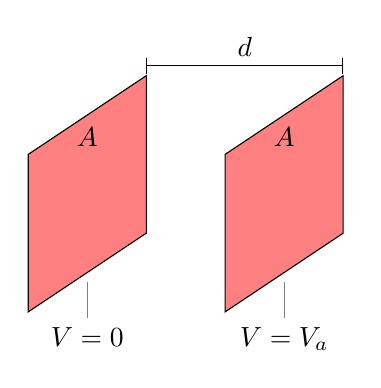
\begin{tikzpicture}
        \draw [fill=red!50]
          (0,0)
          -- node[below=1]{$A$}
            node(plate1)[above,pos=1]{}
            ++(1.5,1)
          -- ++(0,-2)
          -- node[pin={below:$V=0$}]{} ++(-1.5,-1)
          -- cycle
        ;
        \draw [fill=red!50]
          (2.5,0)
          -- node[below=1]{$A$}
            node(plate2)[above,pos=1]{}
            ++(1.5,1)
          -- ++(0,-2)
          -- node[pin={below:$V=V_a$}]{} ++(-1.5,-1)
          -- cycle
        ;
        \draw[|-|]
          (plate1.center)
          -- node[above]{$d$} (plate2.center);
      \end{tikzpicture}
    \end{figure}
  \end{column}
\end{columns}
\begin{block}{Child-Langmuir Law}
  \begin{equation*}
    I_a  = JA = \frac{4 \varepsilon_0}{9}\sqrt{\frac{2 e}{m_e} } \frac{A V_a^{3/2}}{d^2}
  \end{equation*}
\end{block}
\end{frame}

\begin{frame}{Quantum Step Approximation}
	\begin{columns}
	\begin{column}{.48 \linewidth}
    We have the relations:
    	\begin{itemize}
          \item $ k_{0 \smallT} = k_{1 \smallT} $
          \item<2-> Trigonometric Identities
          \item<3-> 1D Transmission result: \\ $ T(k(E),\theta) =
          \frac{4 k_{0 z} k_{1 z}}{ \left ( k_{0 z} + k_{1 z} \right ) ^{2} } $
        \end{itemize}    
  	\end{column}
	\begin{column}{.52 \linewidth}
    	\begin{figure}[H]
          	\centering
        	\shadowbox
        	{
        	\only<article| beamer>{
        	\only<1-3>{
        	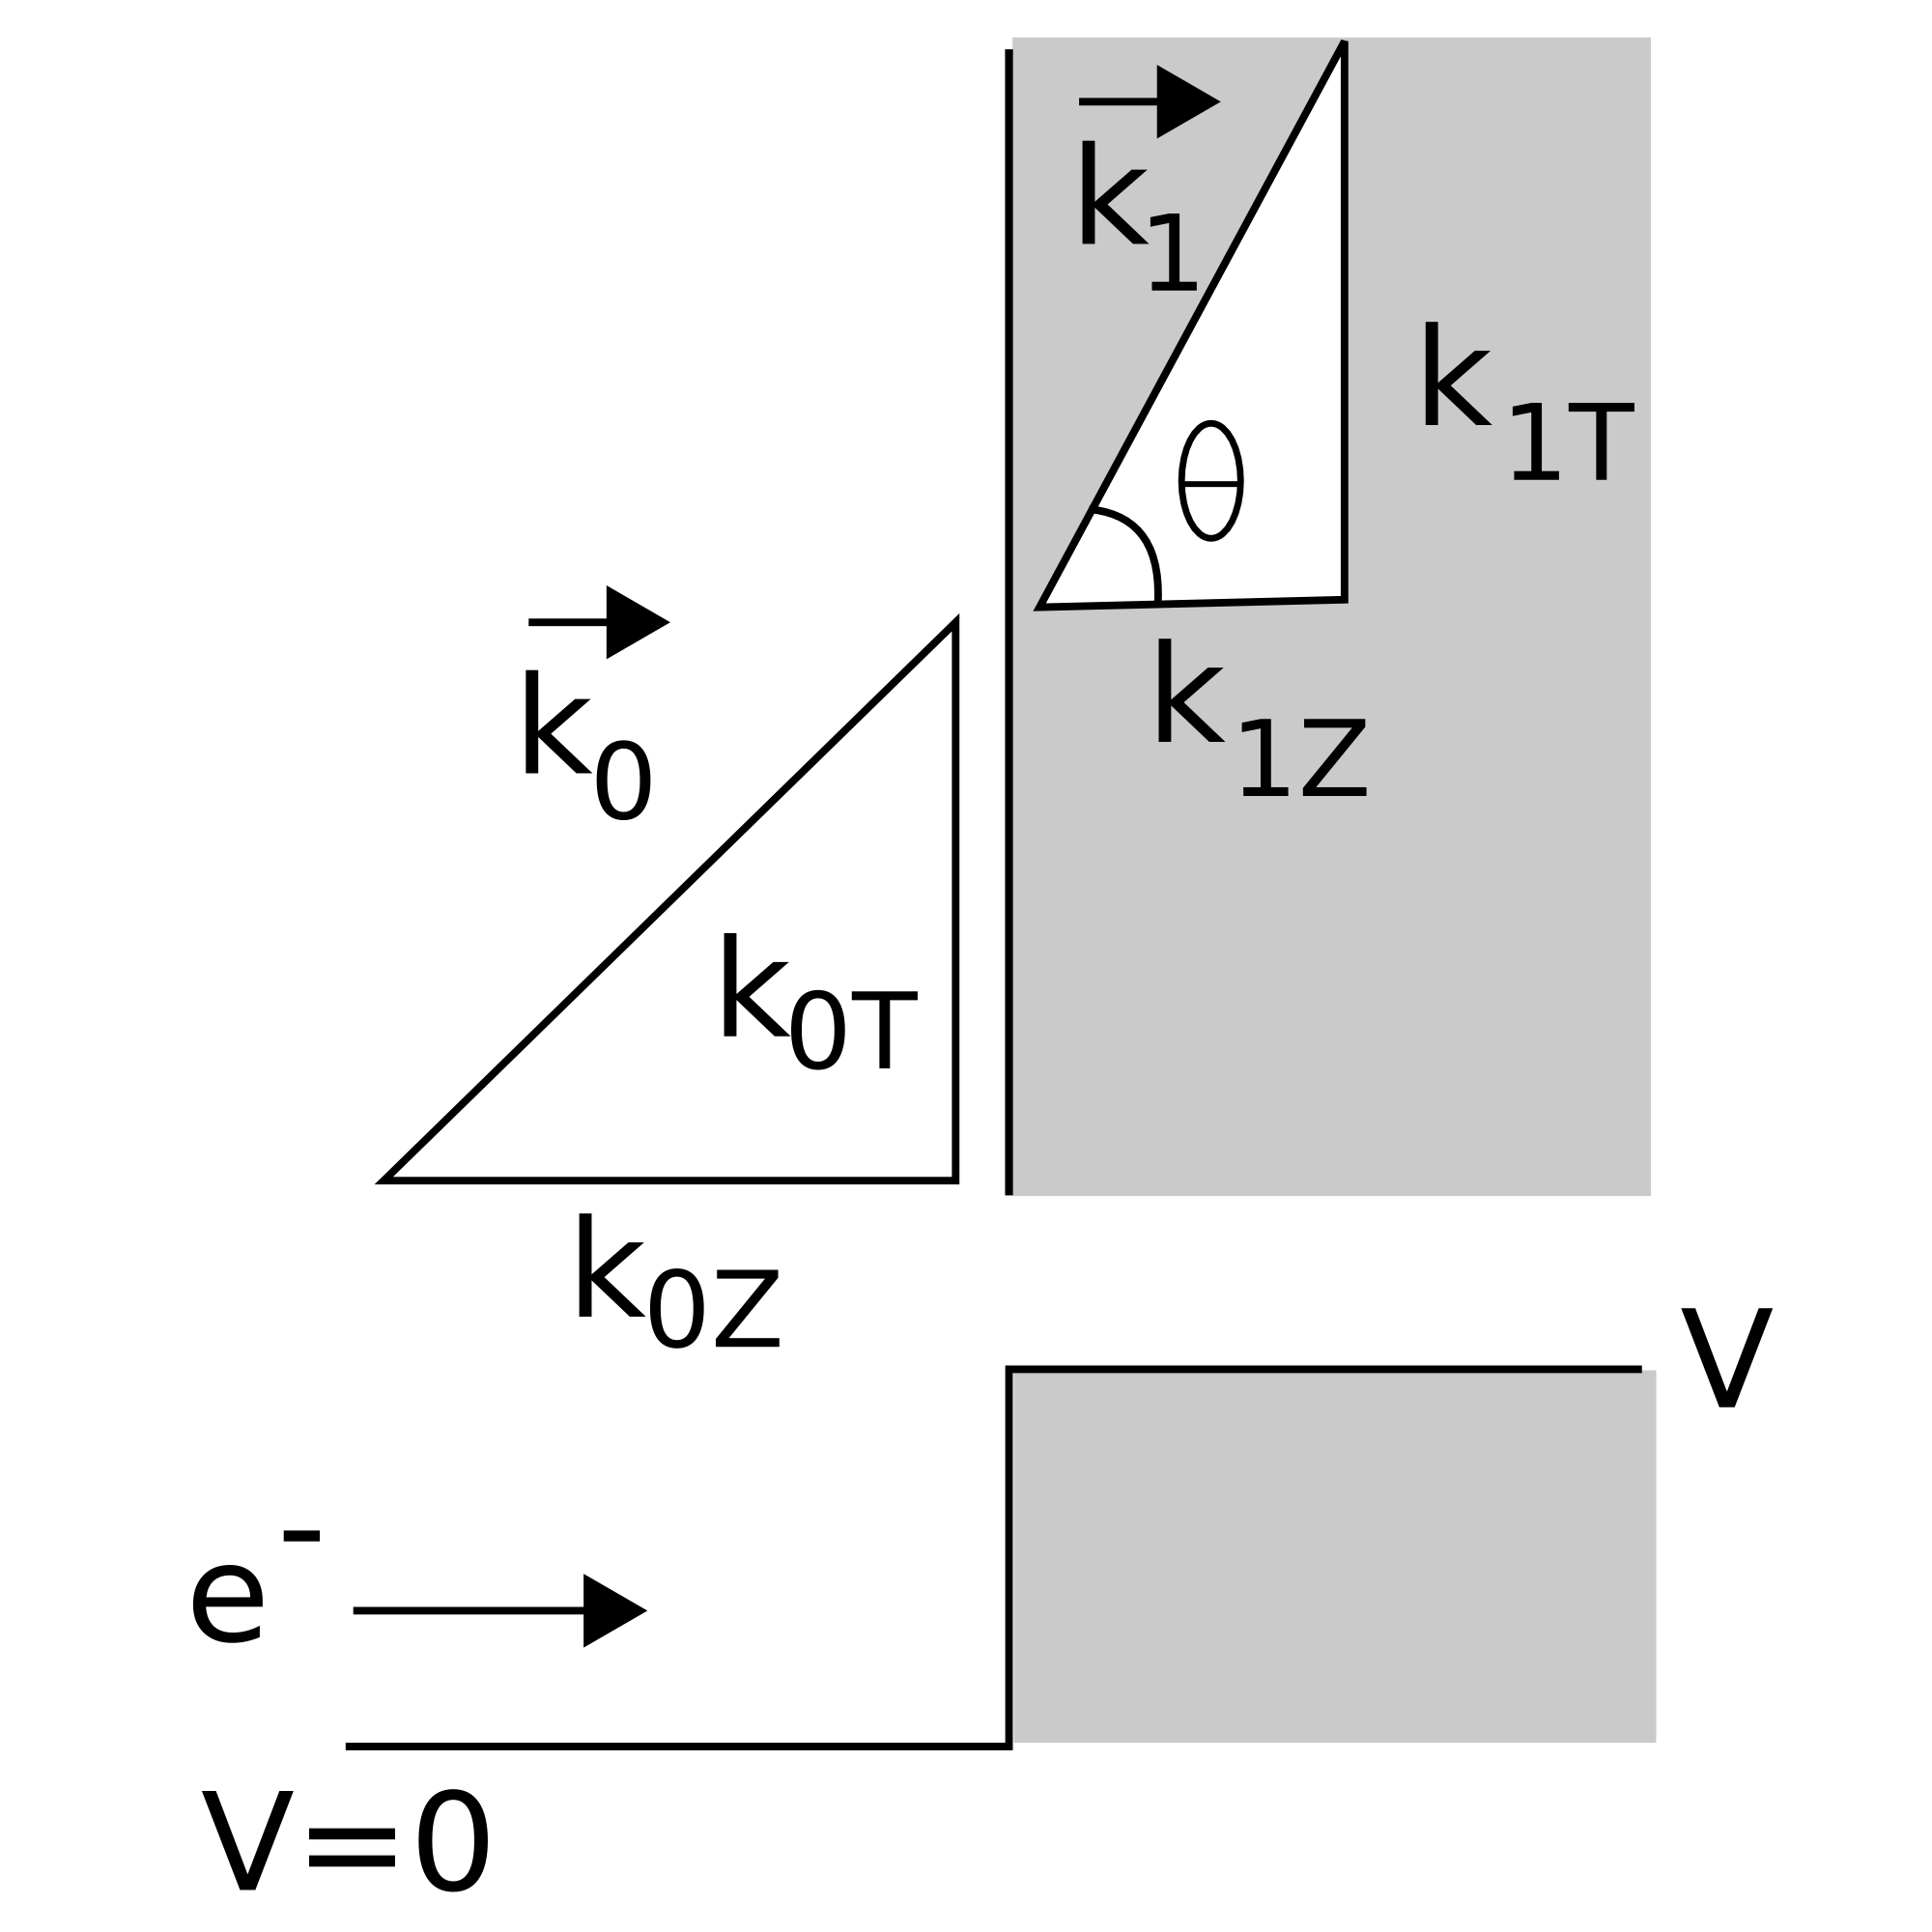
\includegraphics{quantum_step}
        	}}
        	\only<presentation>{
        	\only<4->{
        	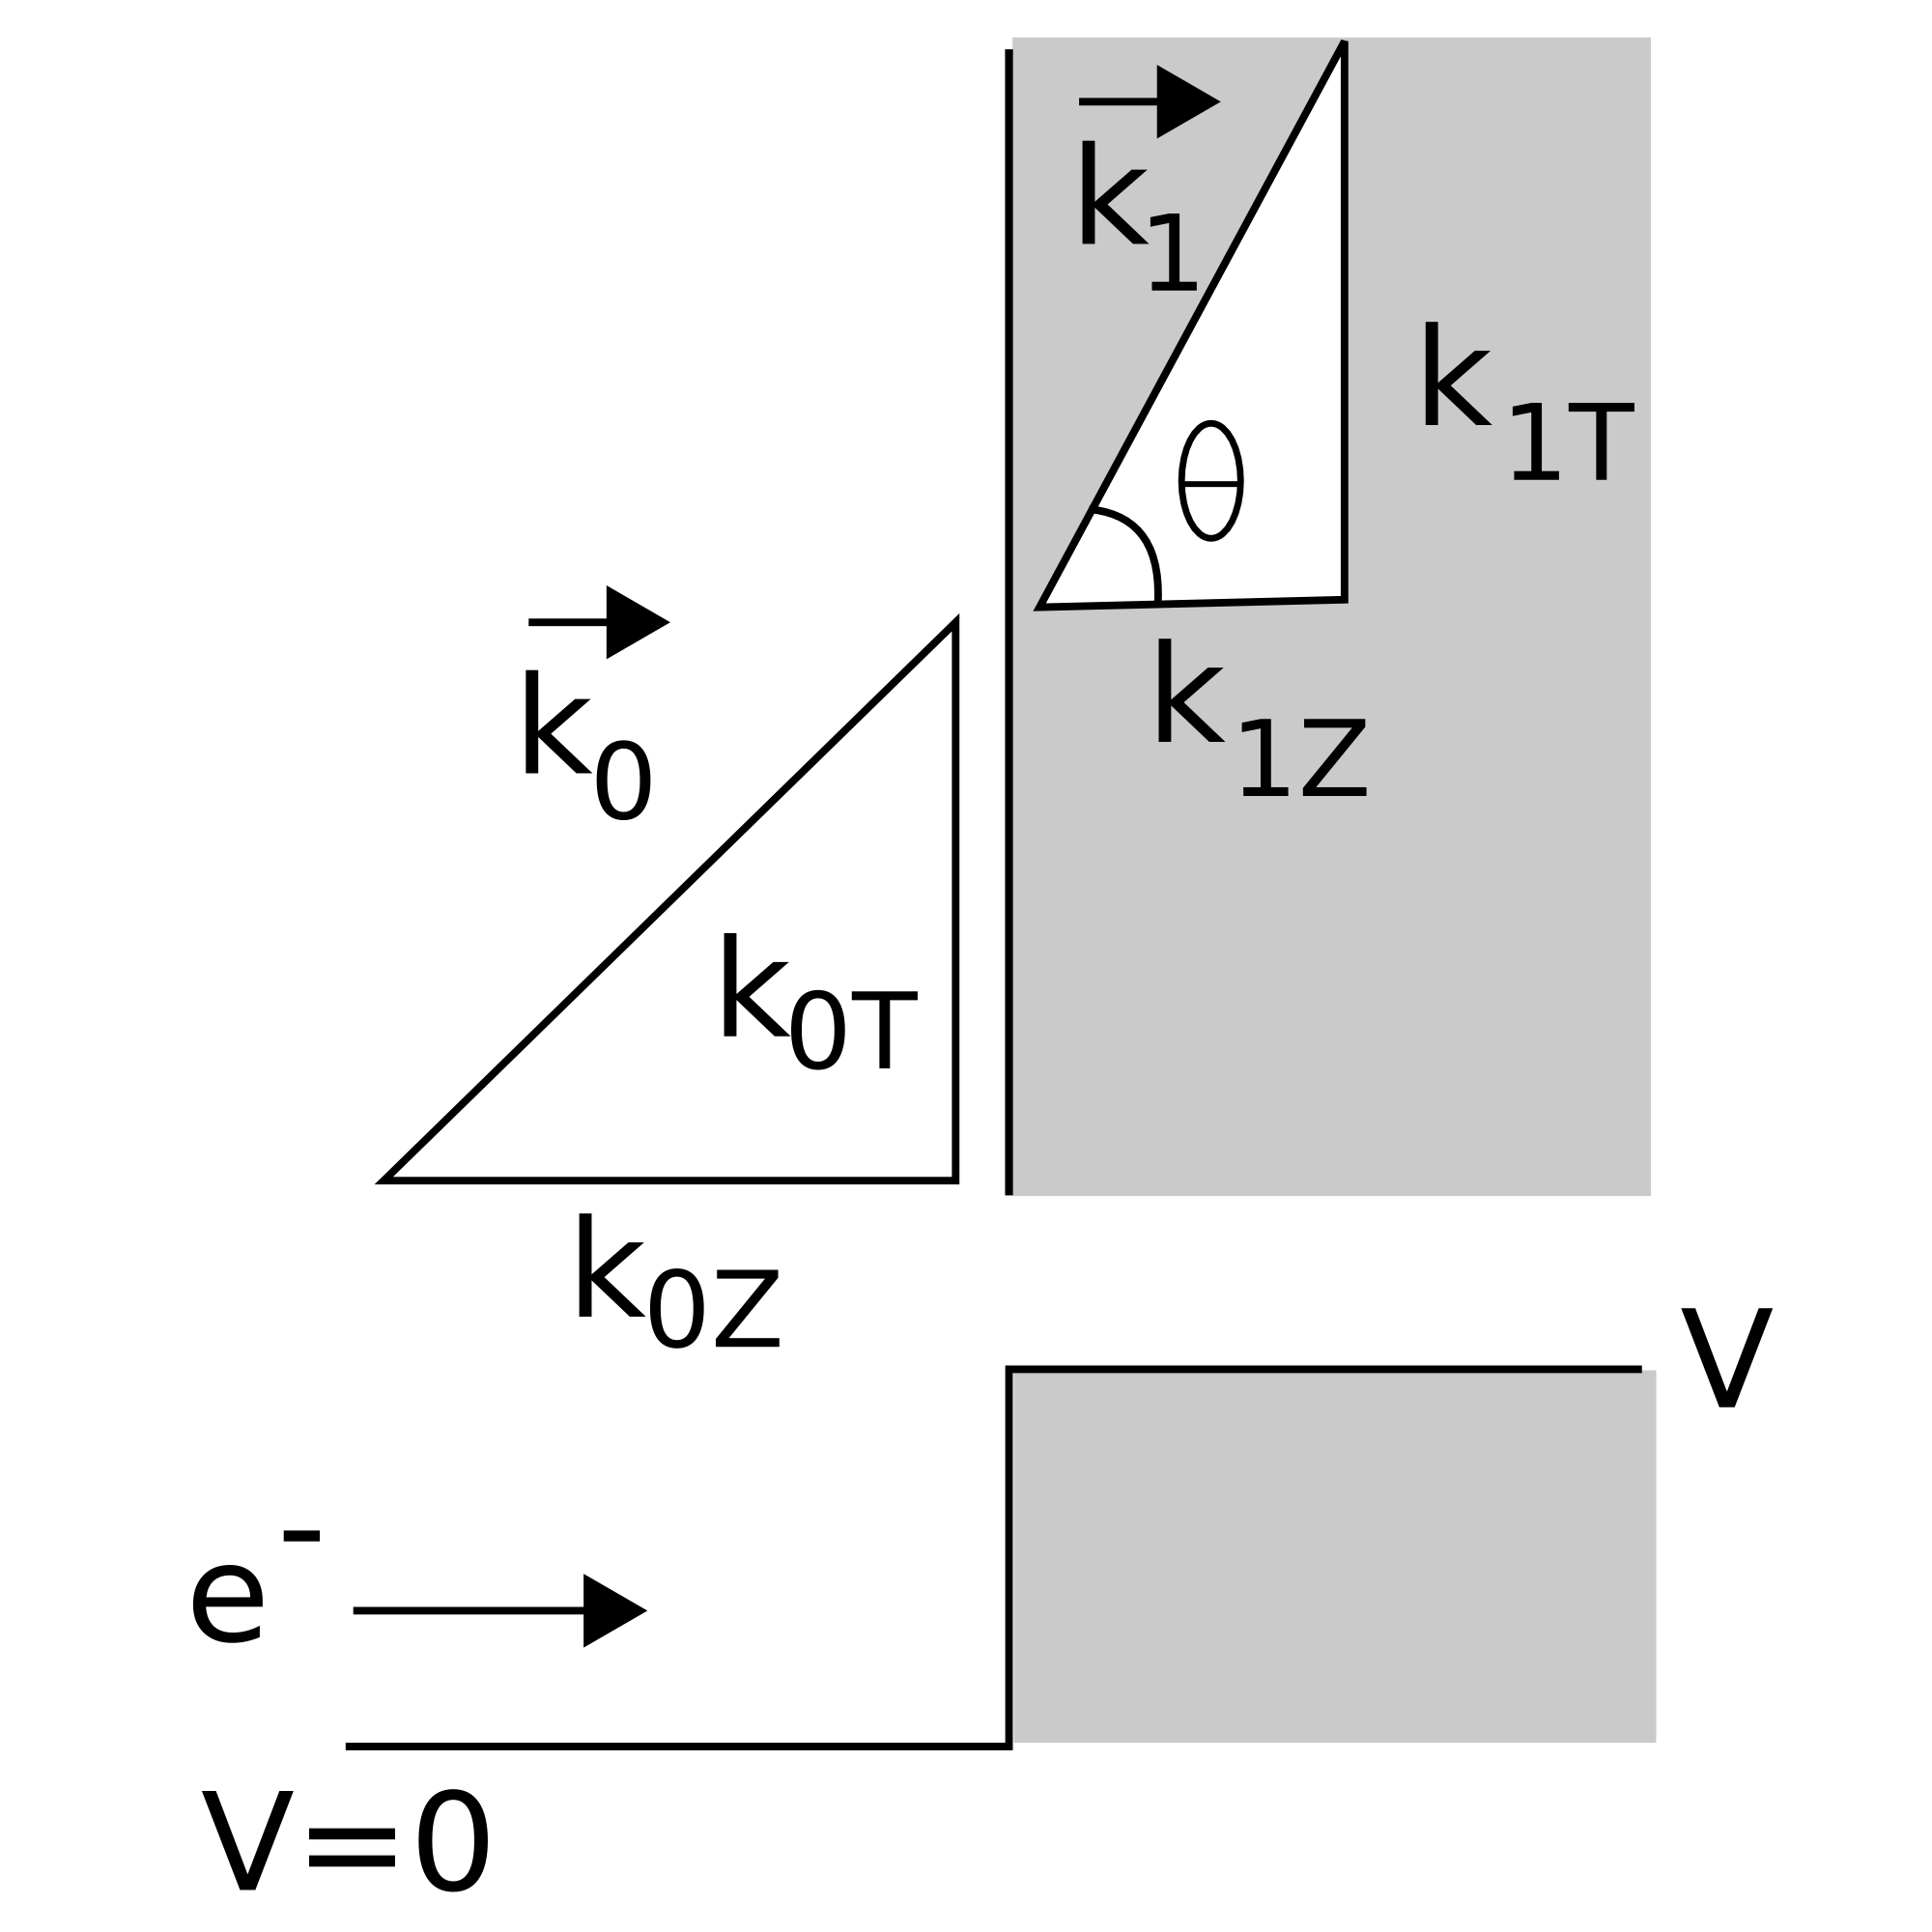
\includegraphics[scale=0.7]{quantum_step}}
        	}}
        	\only<article>{\caption{Quantum Step Potential}}
        \end{figure}
    \end{column}
	\end{columns}
\only<4->
{
    \begin{block}{Resulting Transmission Function}
        \begin{equation*}
           	T(E,\theta) = \frac{4 \sqrt{E} \cos \theta \sqrt{E \cos^{2} \theta
           	+ V } }{ \left ( \sqrt{E} \cos \theta + \sqrt{E \cos^{2} \theta
           	+ V } \right )^{2} }
    	\end{equation*}
		\center{In terms of exit energy $E$ and exit angle $\theta$}
    \end{block}
}
\end{frame}

\begin{frame}{Photoemission from Flat Metal}
  \begin{columns}
  \begin{column}{0.54\linewidth}
  \begin{center}
  \begin{tikzpicture}
    \filldraw
      [fill=black!50]
      (0,0) 
      node [name=photocathode1,below right]{}
      node [below=1mm of photocathode1] {}
      -- ++(1,0)
      -- ++(0,-5)
      node [name=source,midway] {} 
      -- ++(-1,0)
      -- cycle
    ;
    \draw
      [-latex,ultra thick,green] 
      ($(source) + (45:3.5)$) 
      -- (source.east)
      node [name=laser label,pos=0.3,black,fill=white] {Laser ($\lambda$)}
    ;
    \fill
      [blue!30]
      (source.east)
      -- ++(3,6mm)
      -- ++(0,-12mm)
      -- cycle
    ;
    \draw
      [-latex,ultra thick,blue]
      (source.east)
      -- ++(3,6mm)
    ;
    \draw
      [-latex,ultra thick,blue]
      (source.east)
      -- ++(3,-6mm)
      node [name=electron label,at end,black,below,align=center]{Photoemitted\\Electrons}
    ;
    \draw
      [dashed]
      (source)
      -- ++(4,0)
    ;
%     \draw 
%       ($(source) + (1,0)$) 
%       arc (0:41:1)
%       node [right=0.3] {$\theta$}
%     ;
  \end{tikzpicture}
  \end{center}
  \end{column}
  \begin{column}{0.44\linewidth}
    \begin{equation*}
      P(\theta) = \smashoperator{\int\limits_{0}^{\Delta E = \hbar \omega - \Phi}} T(E,\theta) \dx{E}
    \end{equation*}
    \centerline{\tiny Assuming flat Fermi function}
    \begin{figure}
      \centering
      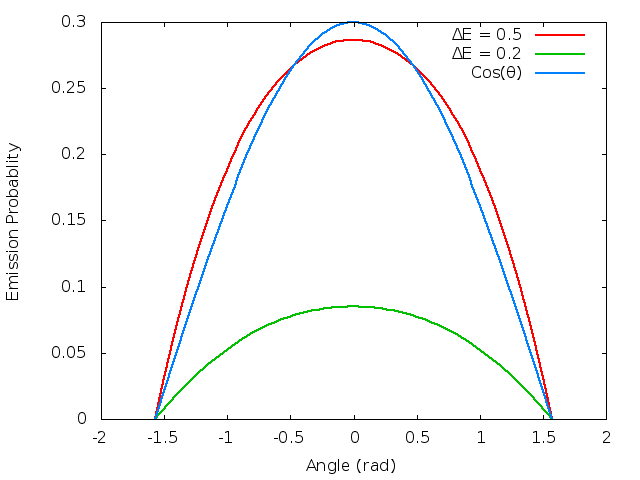
\includegraphics[width=0.9\linewidth]{Angle}
    \end{figure}
  \end{column}
  \end{columns}
\end{frame}

\begin{frame}{Emission Probability vs. Excess Energy}
  \begin{columns}
    \begin{column}{0.49\linewidth}
      %Angularly-integrated Emission Probability
      \begin{equation*}
        P(E) = \int\limits_0^E \int\limits_{-\pi/2}^{-\pi/2} T(E_0,\theta) \dx{\theta}\dx{E_0}
      \end{equation*}
    \end{column}
    \begin{column}{0.49\linewidth}
      \begin{figure}
        \centering
        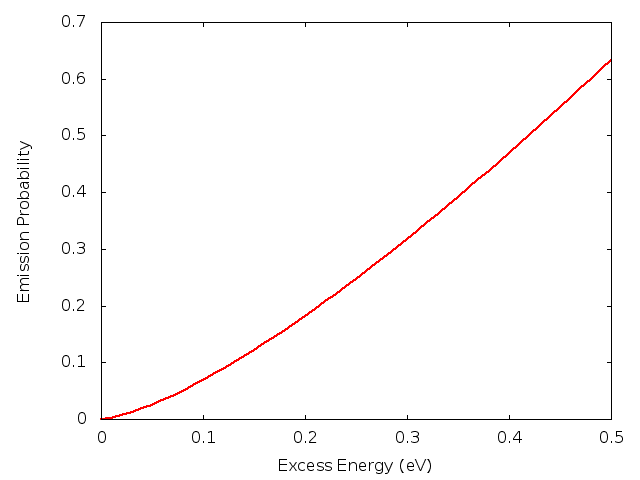
\includegraphics[width=0.9\linewidth]{Energy}
      \end{figure}
    \end{column}
  \end{columns}
  
\end{frame}

\begin{frame}{Gaussian Distribution}
If we define our distribution of electrons in the pulse as:
	\begin{multline*}
		f \left ( x , y , z , p_{x} , p_{y} , p_{z} \right ) = \\ \frac{N}{ \left ( 2 \pi \right )^{3} \sigma_{ \smallT } \eta_{ \scriptscriptstyle T } \sqrt{ \sigma_{z} \eta_{z}} } \exp \Biggl [ - \biggl ( \frac{x^{2}} {2 \sigma_{ \smallT }} + \frac{y^{2}} {2 \sigma_{ \smallT }} + \frac{z^{2}} {2\sigma_{z}} + \\ \frac{ \left ( p_{x} - \dfrac{\gamma_{ \smallT } x} {\sigma_{ \smallT }} \right )^{2}} {2 \eta_{ \smallT }} + \frac{ \left ( p_{y} - \dfrac{\gamma_{ \smallT } y} {\sigma_{ \smallT }} \right )^{2}} {2 \eta_{ \smallT }} + \frac{ \left (p_{z} - \dfrac{\gamma_{z} z} {\sigma_{z}} \right )^{2}} {2 \eta_{z}} \biggr ) \Biggr ]
	\end{multline*}
N.B. the coefficient allows $ \int f d\vec{r} d\vec{p} = N $

\end{frame}

\begin{frame}{What Are These Parameters?}
	\begin{columns}
		\begin{column}{2in}
			\begin{itemize}[<+->]
				\item $ \sigma_{i} \Rightarrow$ spatial variance
				\item $ \eta_{i} \Rightarrow$ \emph{local} momentum variance
				\item $ \gamma_{i} \Rightarrow$ spatial variation of the local momentum variance (chirp)
			\end{itemize}
		\end{column}
		\begin{column}{2in}
			\begin{figure}
				\includegraphics<1>{Gaussian1.jpg}
				\includegraphics<2>{Gaussian2.jpg}
				\includegraphics<3>{Gaussian3.jpg}
			\end{figure}
		\end{column}
	\end{columns}
\end{frame}

\begin{frame}{AG Model Equations}
\begin{block}{Michalik and Sipe equation set}
	\begin{gather*}
		\frac{d\sigma_{i}} {dt} = \frac{2} {m} \gamma_{i} \\
		\frac{d \gamma_{i}} {dt} = \frac{1} {m} \left (\eta_{i} + \frac{\gamma_{i}^{2}} {\sigma_{i}} \right ) + \frac{1} {4 \pi \epsilon_{0}} \frac{N e^{2}} {6 \sqrt{\sigma_{i} \pi} } L_{i}(\xi) \\
		\frac{d\eta_{i}} {dt} = - \frac{2 \gamma_{i} \eta_{i}} {m \sigma_{i}}
	\end{gather*}
\end{block}
\begin{itemize}
  \item $L_i(\xi)$ are well-behaved smooth functions of $\xi=\sqrt{ \sigma_{z} / \sigma_{t} }$
  \item Solve to classical Gaussian when $ N = 0 $
\end{itemize}
\end{frame}

\begin{frame}{Building the Model}

\begin{columns}
	\begin{column}{.52 \linewidth}
	\begin{itemize}
  		\item<1-> Start with the fastest electron
  		\item<2-> $ v_{fastest} = \sqrt{2 q \Delta E / m } $ \\ $ \Delta E $ is
  		excess photoemission energy
  		\item<3-> Propagate with \\ $ z_{max} = v_{fastest} t_{total} + q E t_{
  		total }^{2} / 2 m $
  		\item<4-> This is the maximum possible range
  		\item<5-> Subdivide the preceding space for future reference
	\end{itemize}
	\end{column}
	
	\begin{column}{.44 \linewidth}
    \begin{overlayarea}{.44 \linewidth}{2.1in}
    \begin{figure}[H]
    	\centering
    	\only<beamer>
    	{
    	\only<1-2>{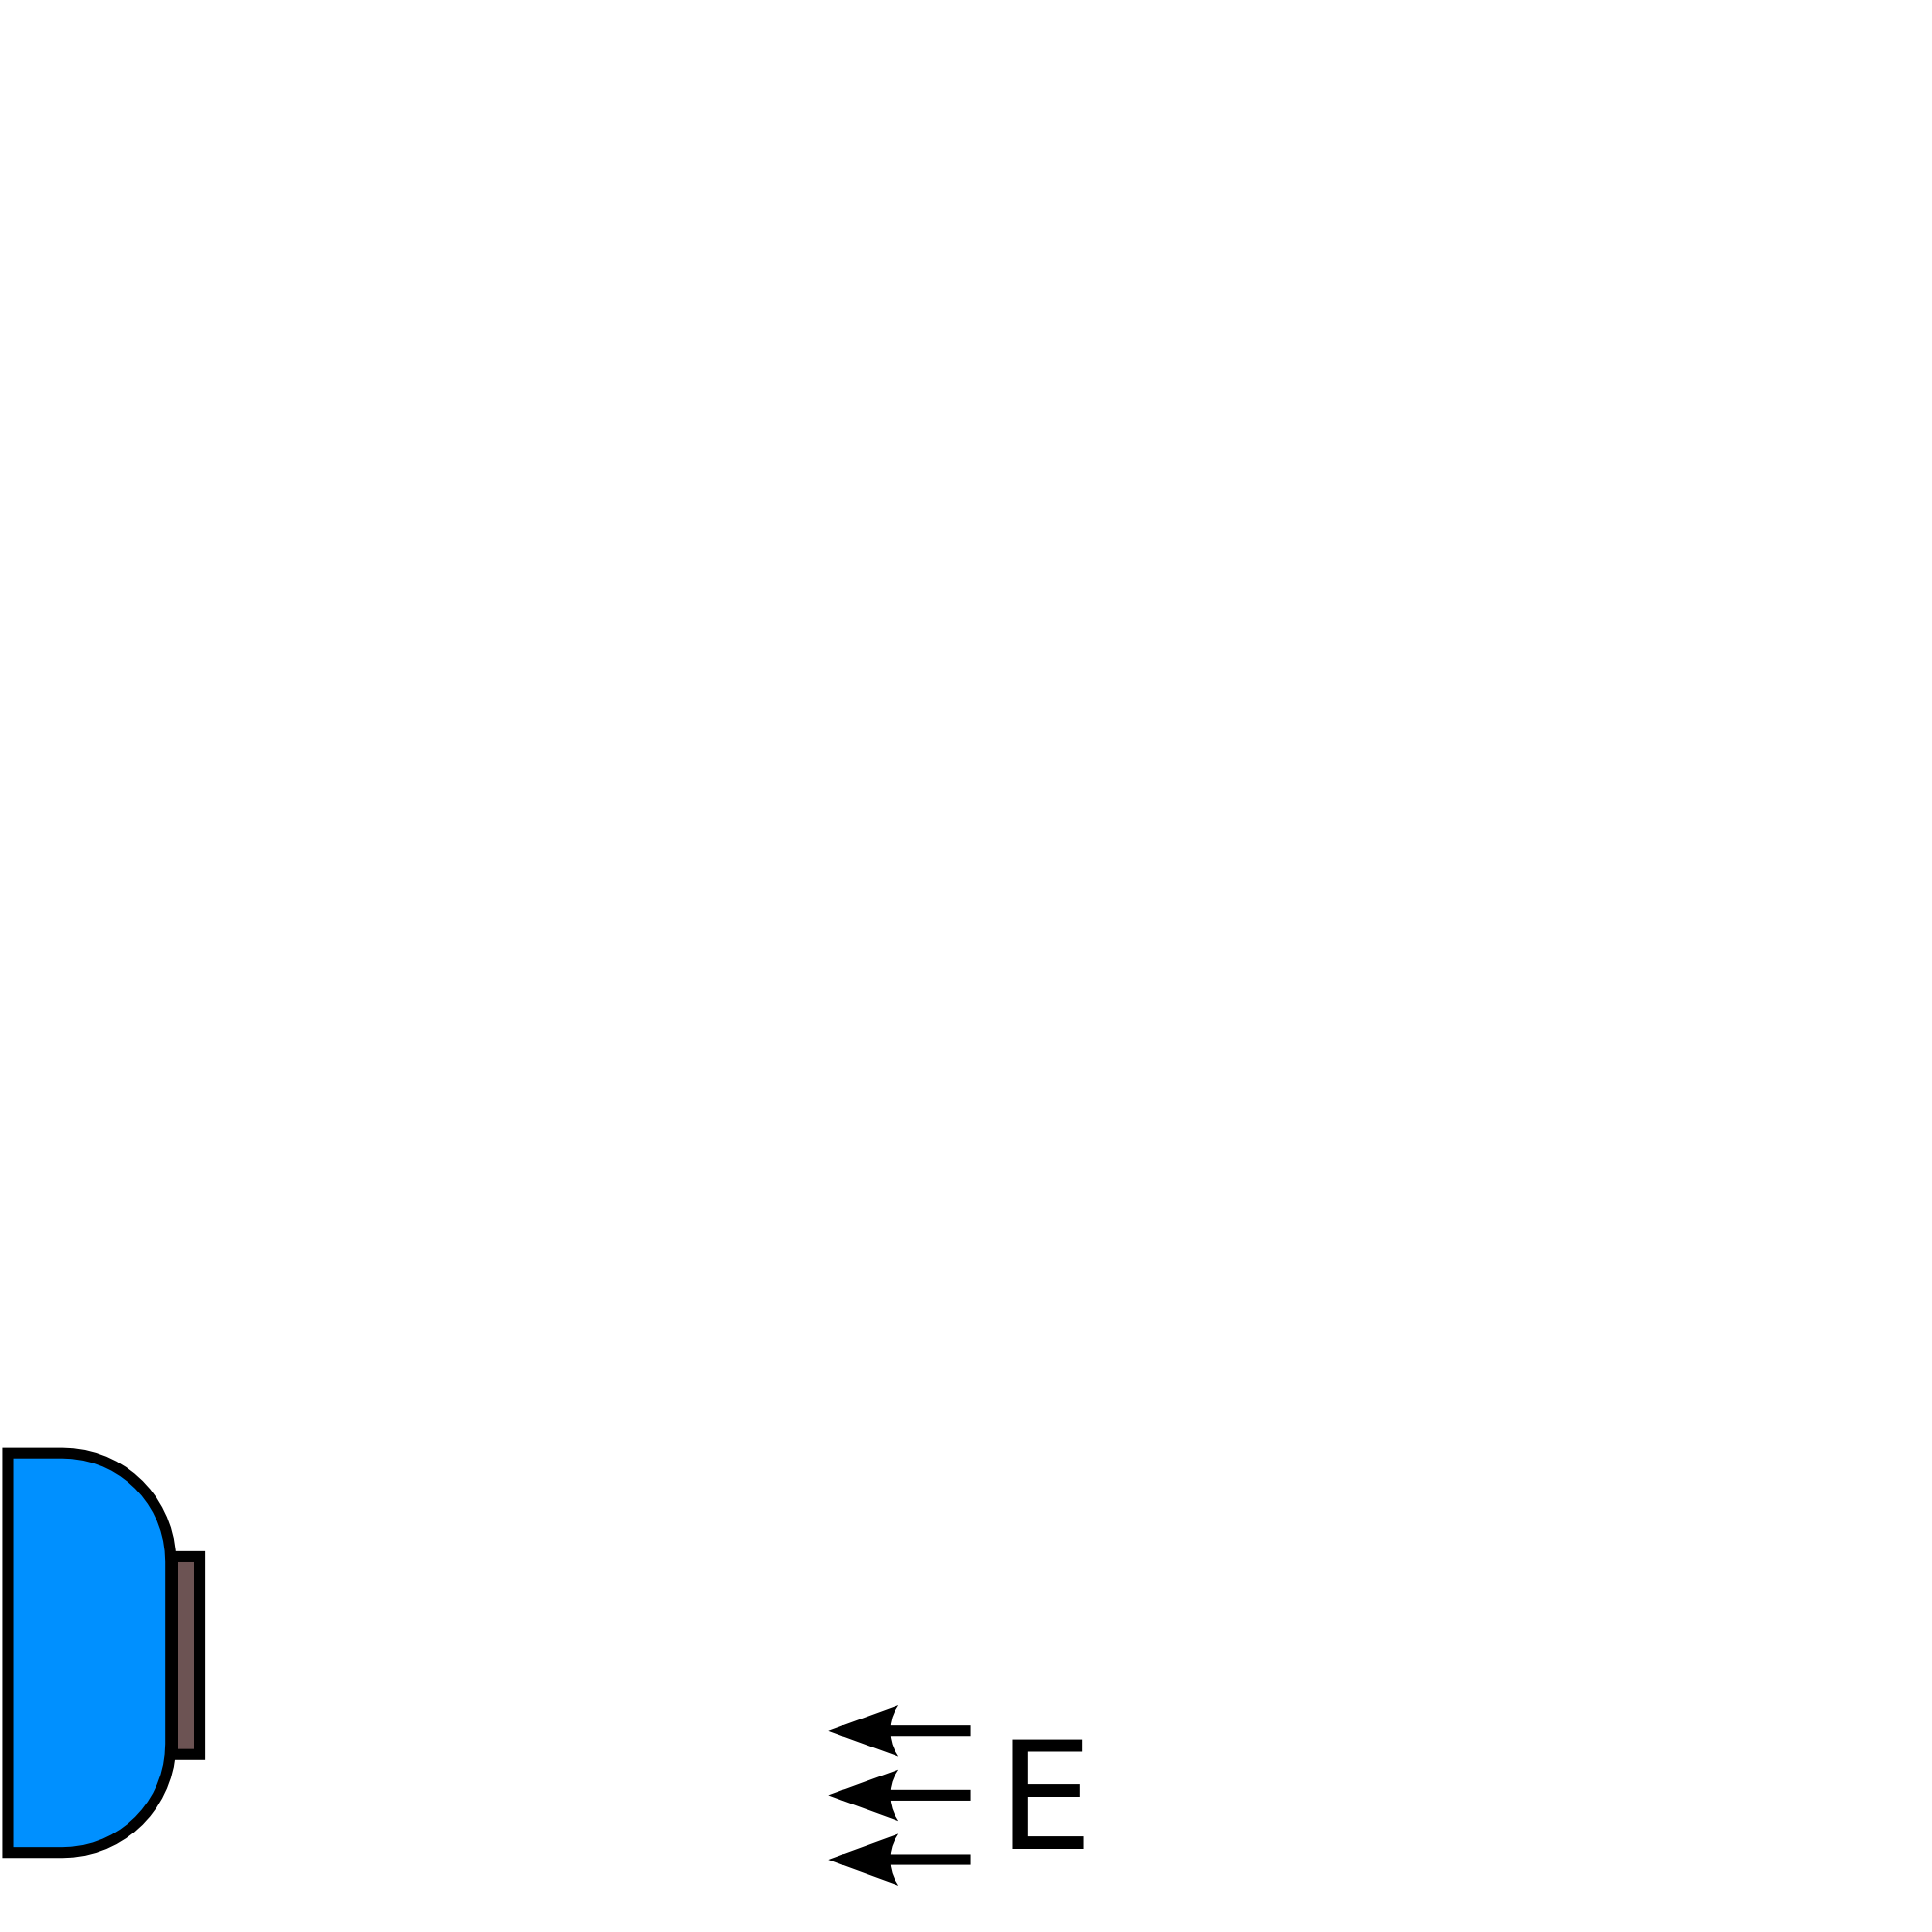
\includegraphics{bin}}
    	\only<3-4>{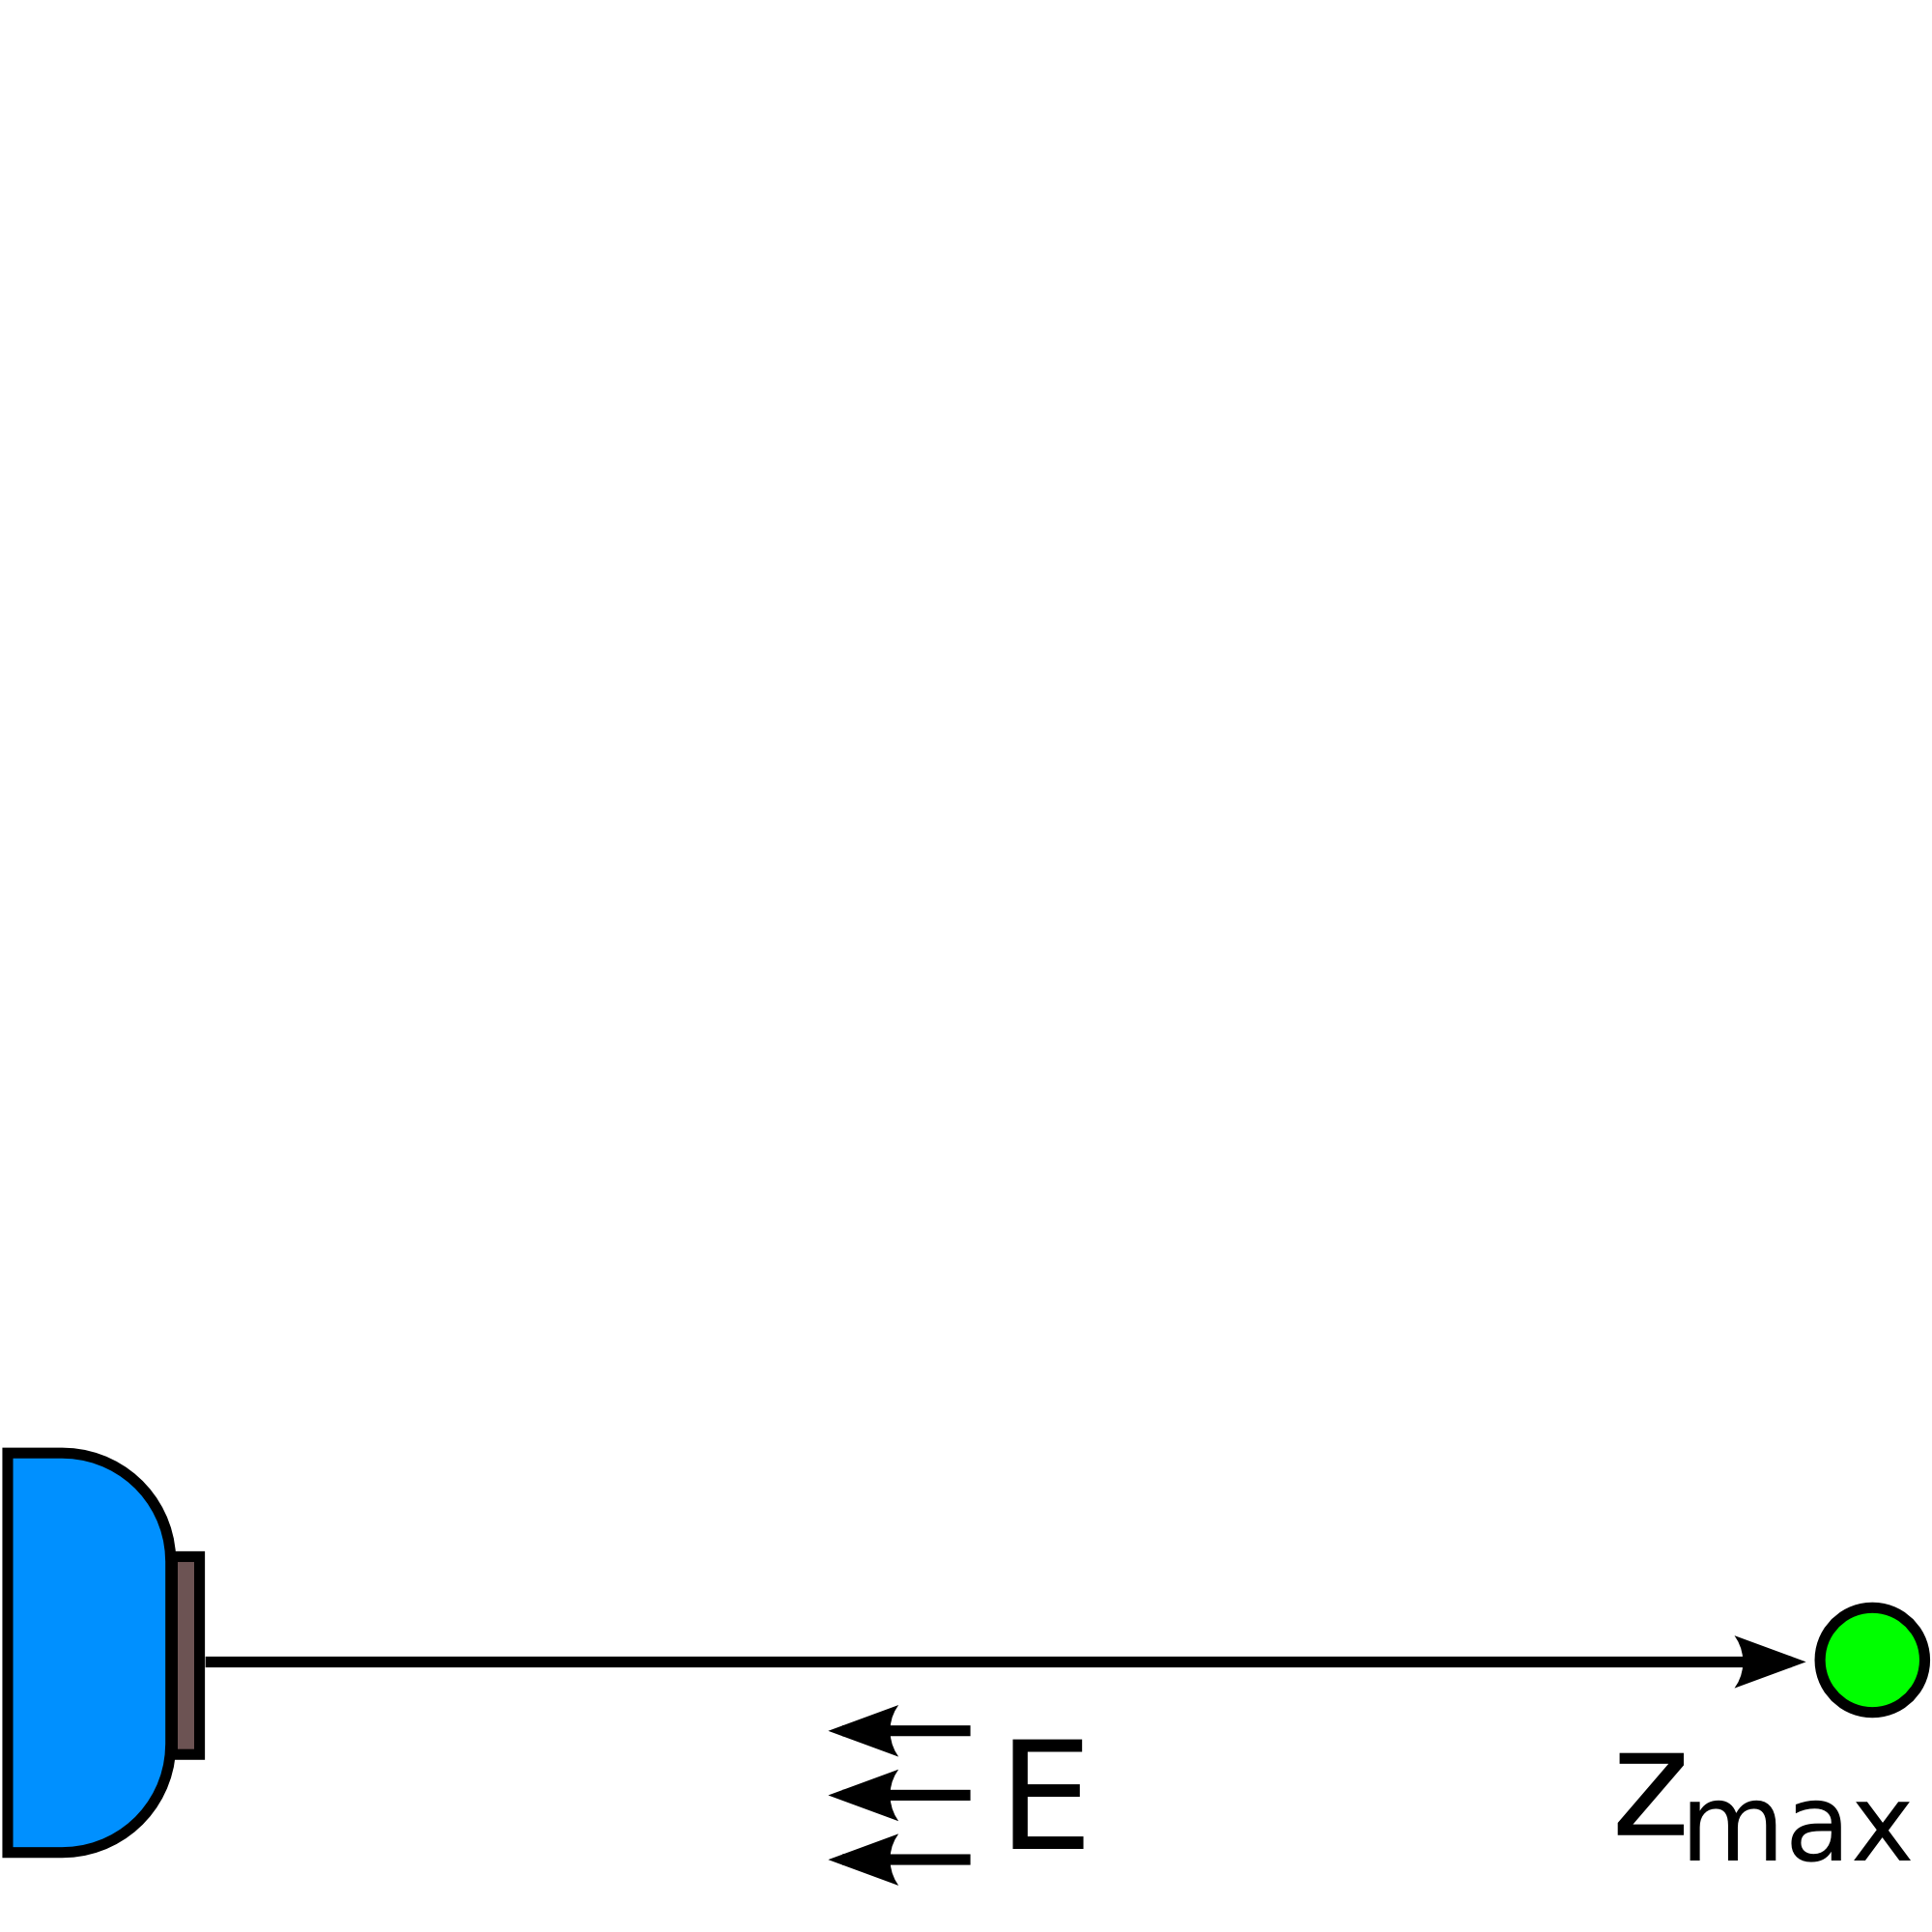
\includegraphics{bin1}}
    	}
    	\only<presentation>{\only<5->{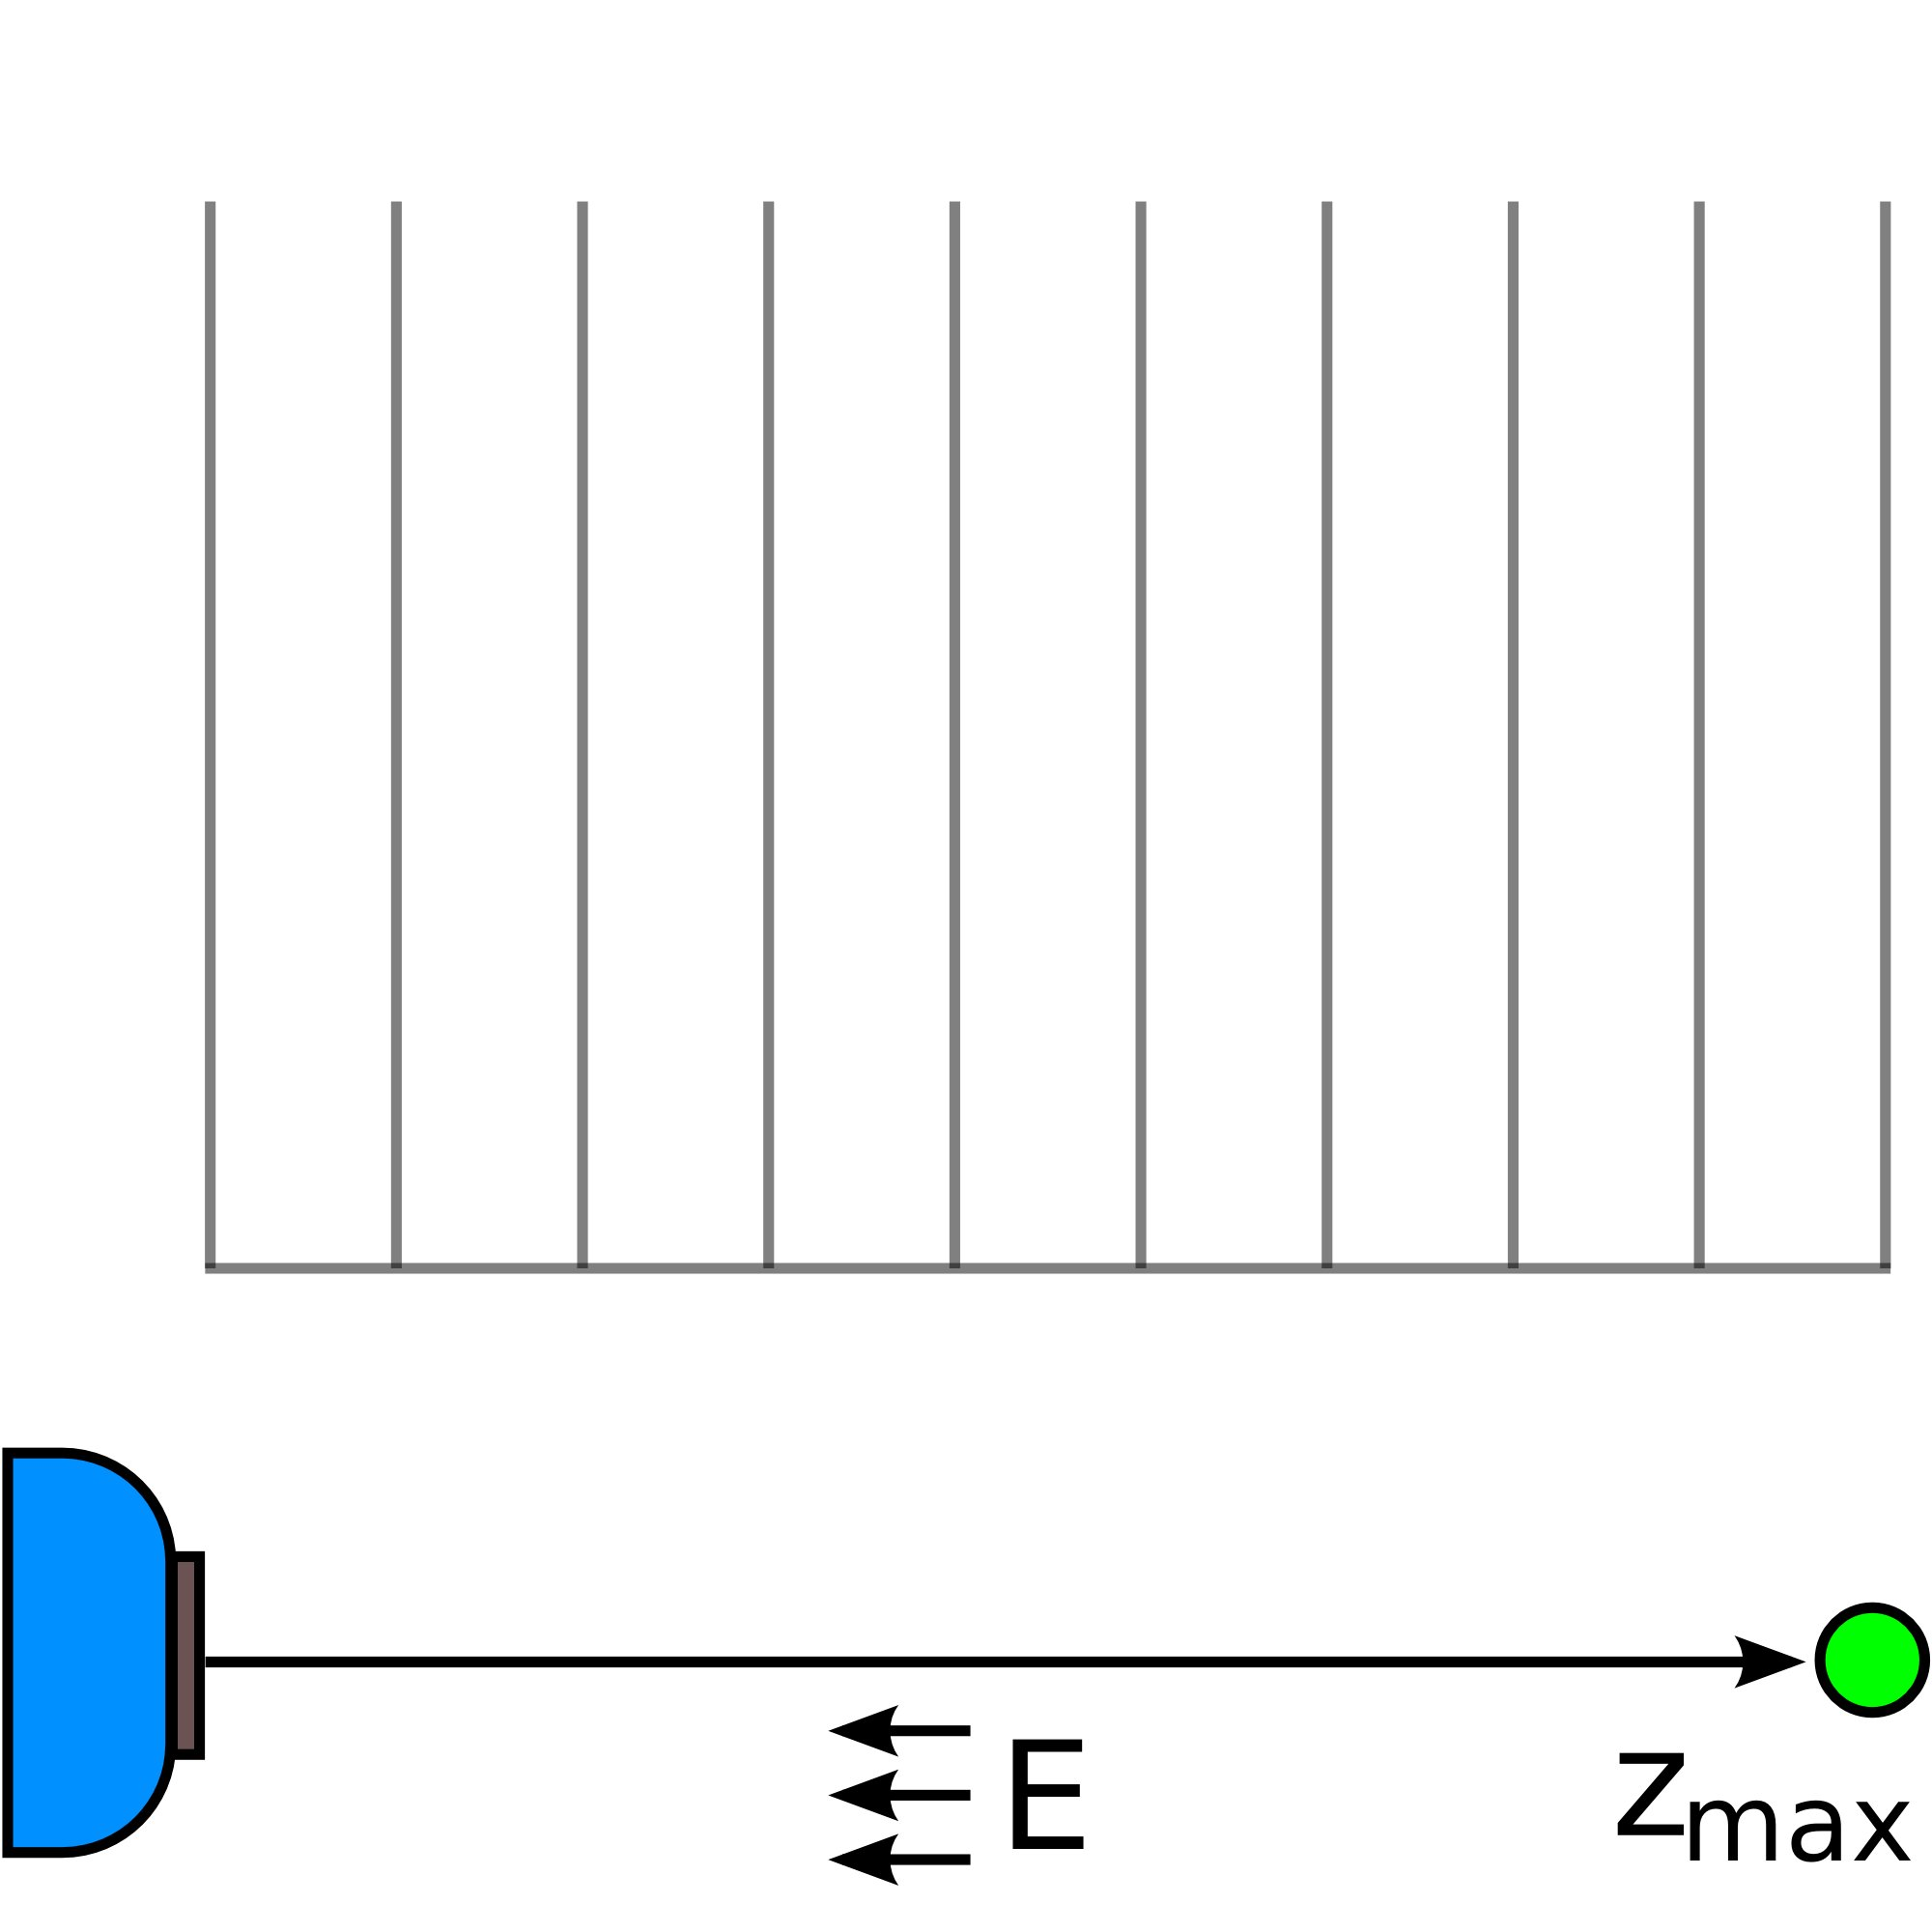
\includegraphics{bin2}}}
    \end{figure}
    \end{overlayarea}
    \end{column}
\end{columns}

\end{frame}

\begin{frame}{Running the Model}

\begin{columns}
	\begin{column}{.52 \linewidth}
	\begin{itemize}
      \item<1-> At each timestep $t_{i}$ label bins by equivalent velocities
      \item<2-> $ v_{ bin } = \frac{ z_{ bin } }{ t_{ i } } - \frac{q E t_{i} }{
      2 m } $ \\ where $ t_{i} =  t_{ total } - i \delta t $
      \item<3-> This allows the velocity distribution to be superimposed
      \item<10-> After all the timesteps the number and velocity distribution
      in each bin can be computed
    \end{itemize}
	\end{column}

	\begin{column}{.44 \linewidth}
    \begin{overlayarea}{.44 \linewidth}{2.1in}
	\begin{figure}[H]
    	\centering
    	\only<beamer>
    	{
    	\only<1-2>{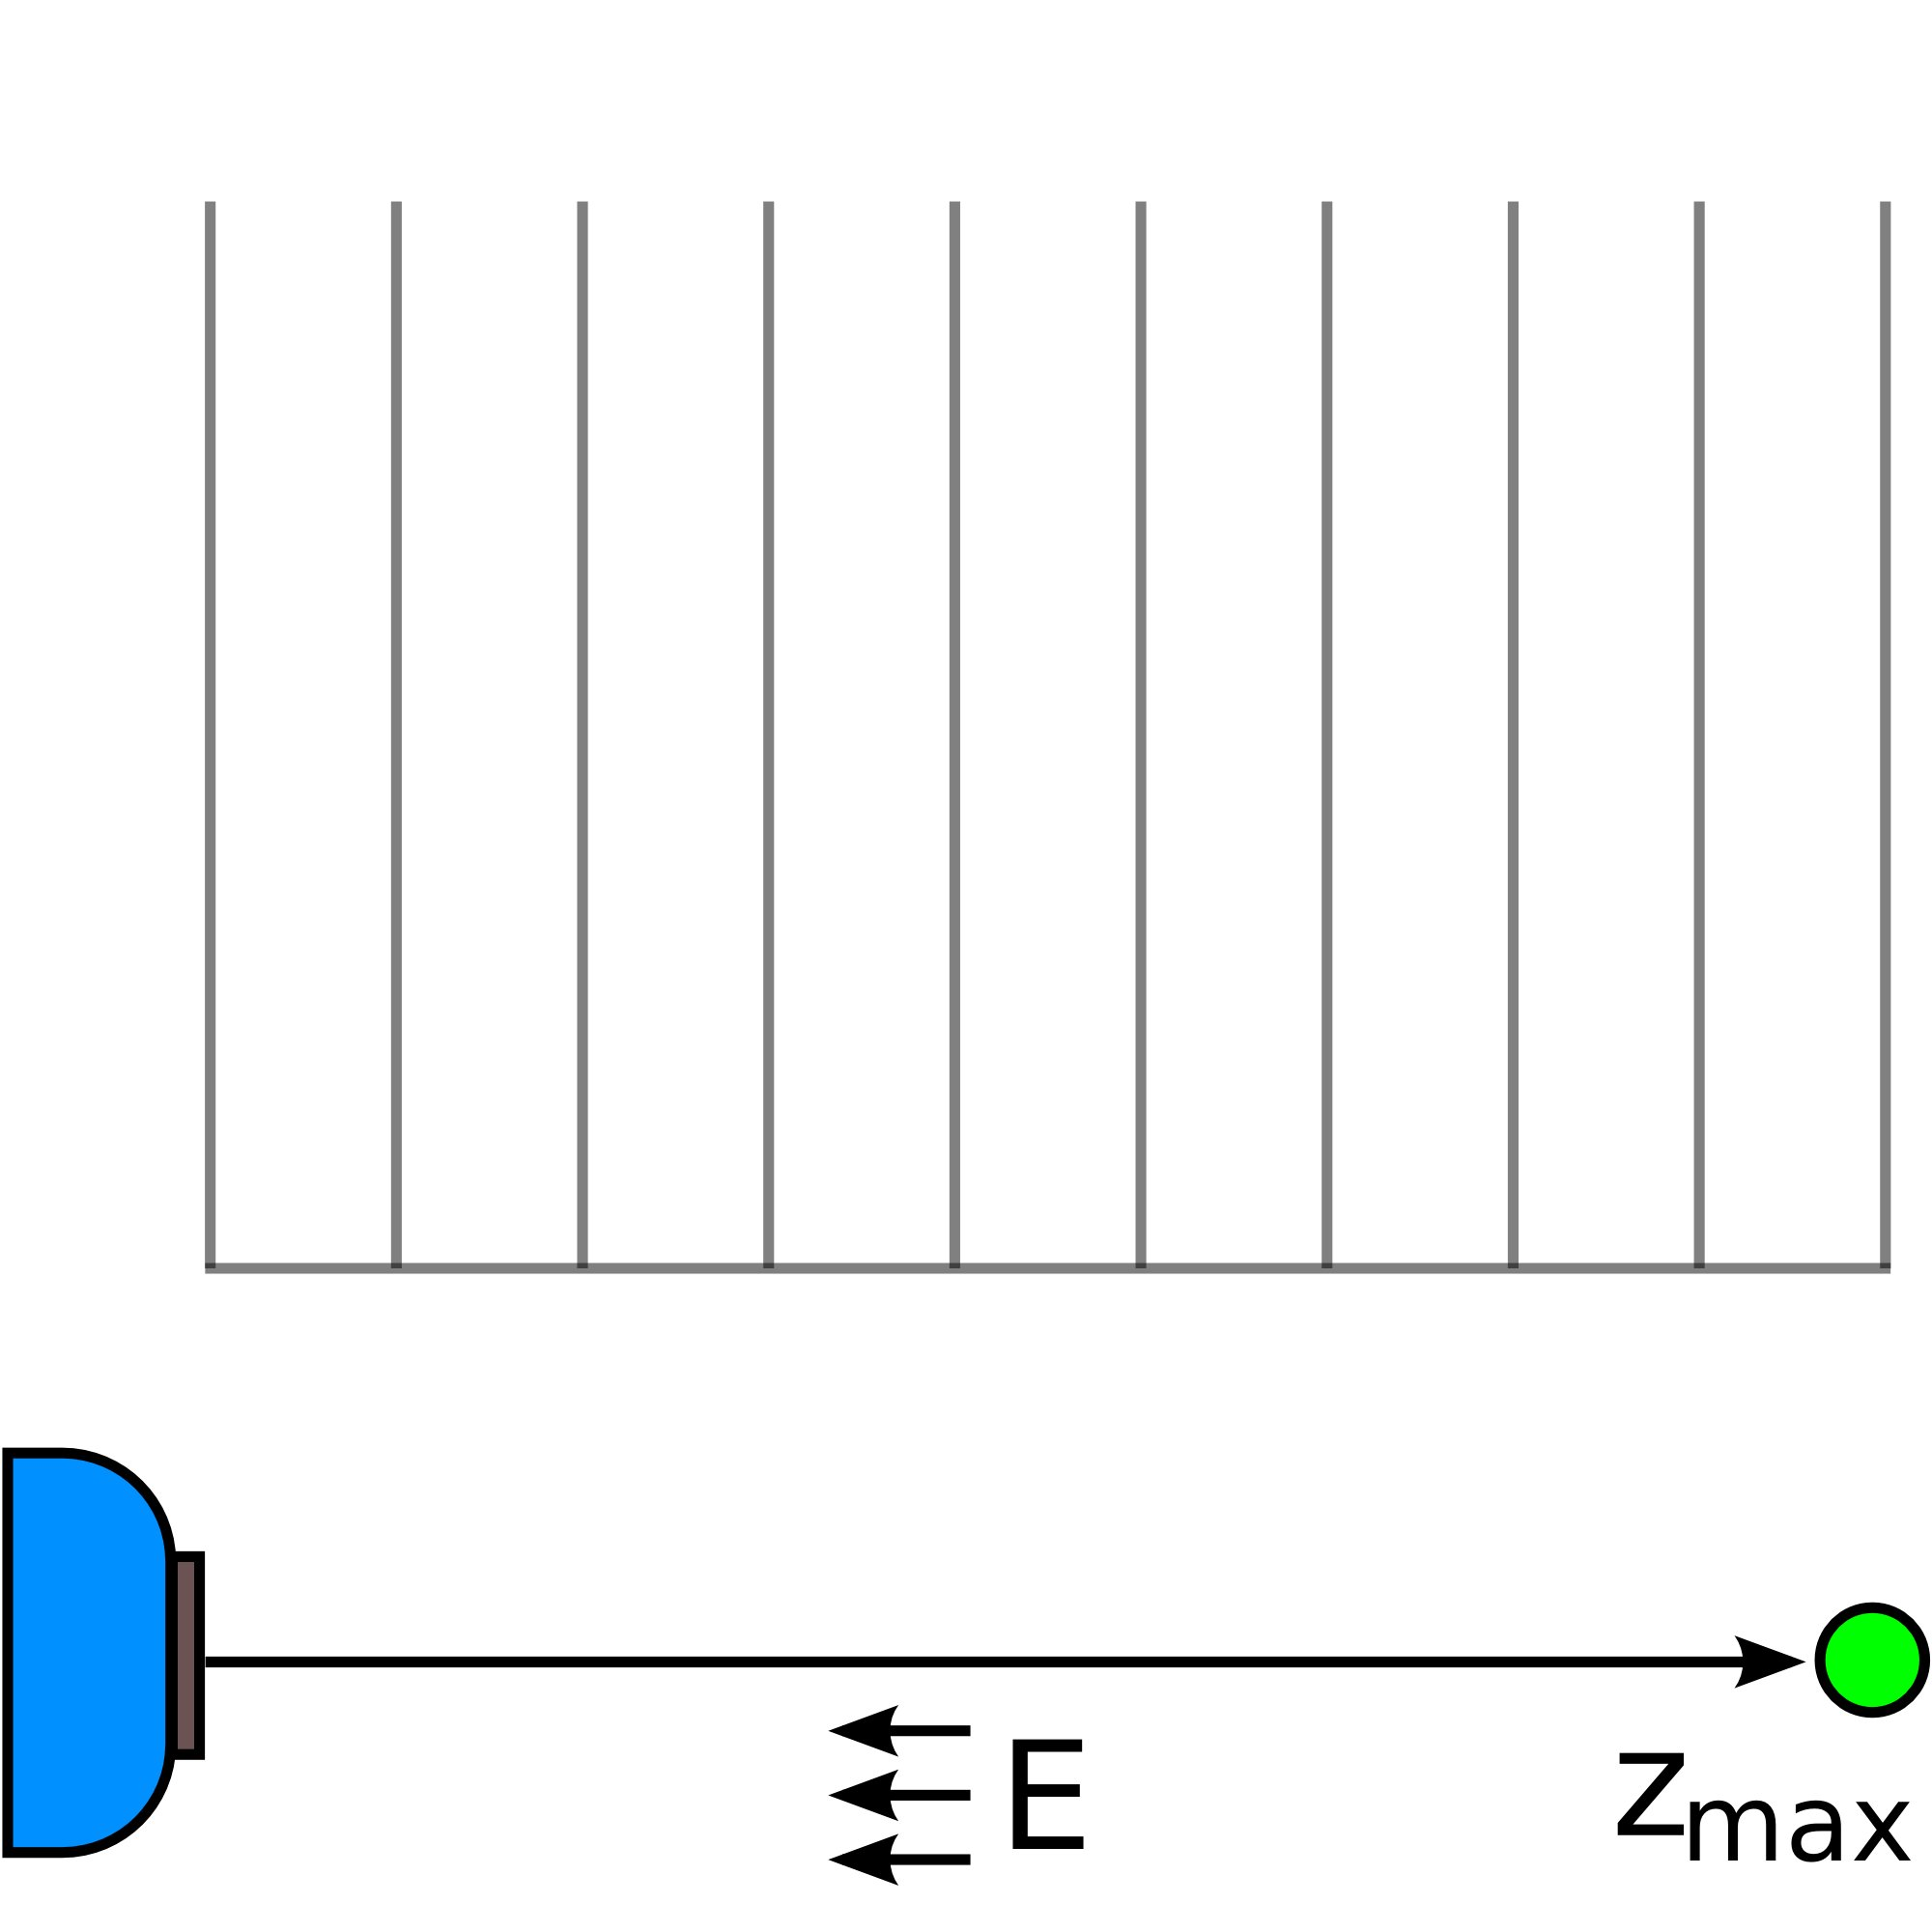
\includegraphics{bin2}}
    	\only<3>{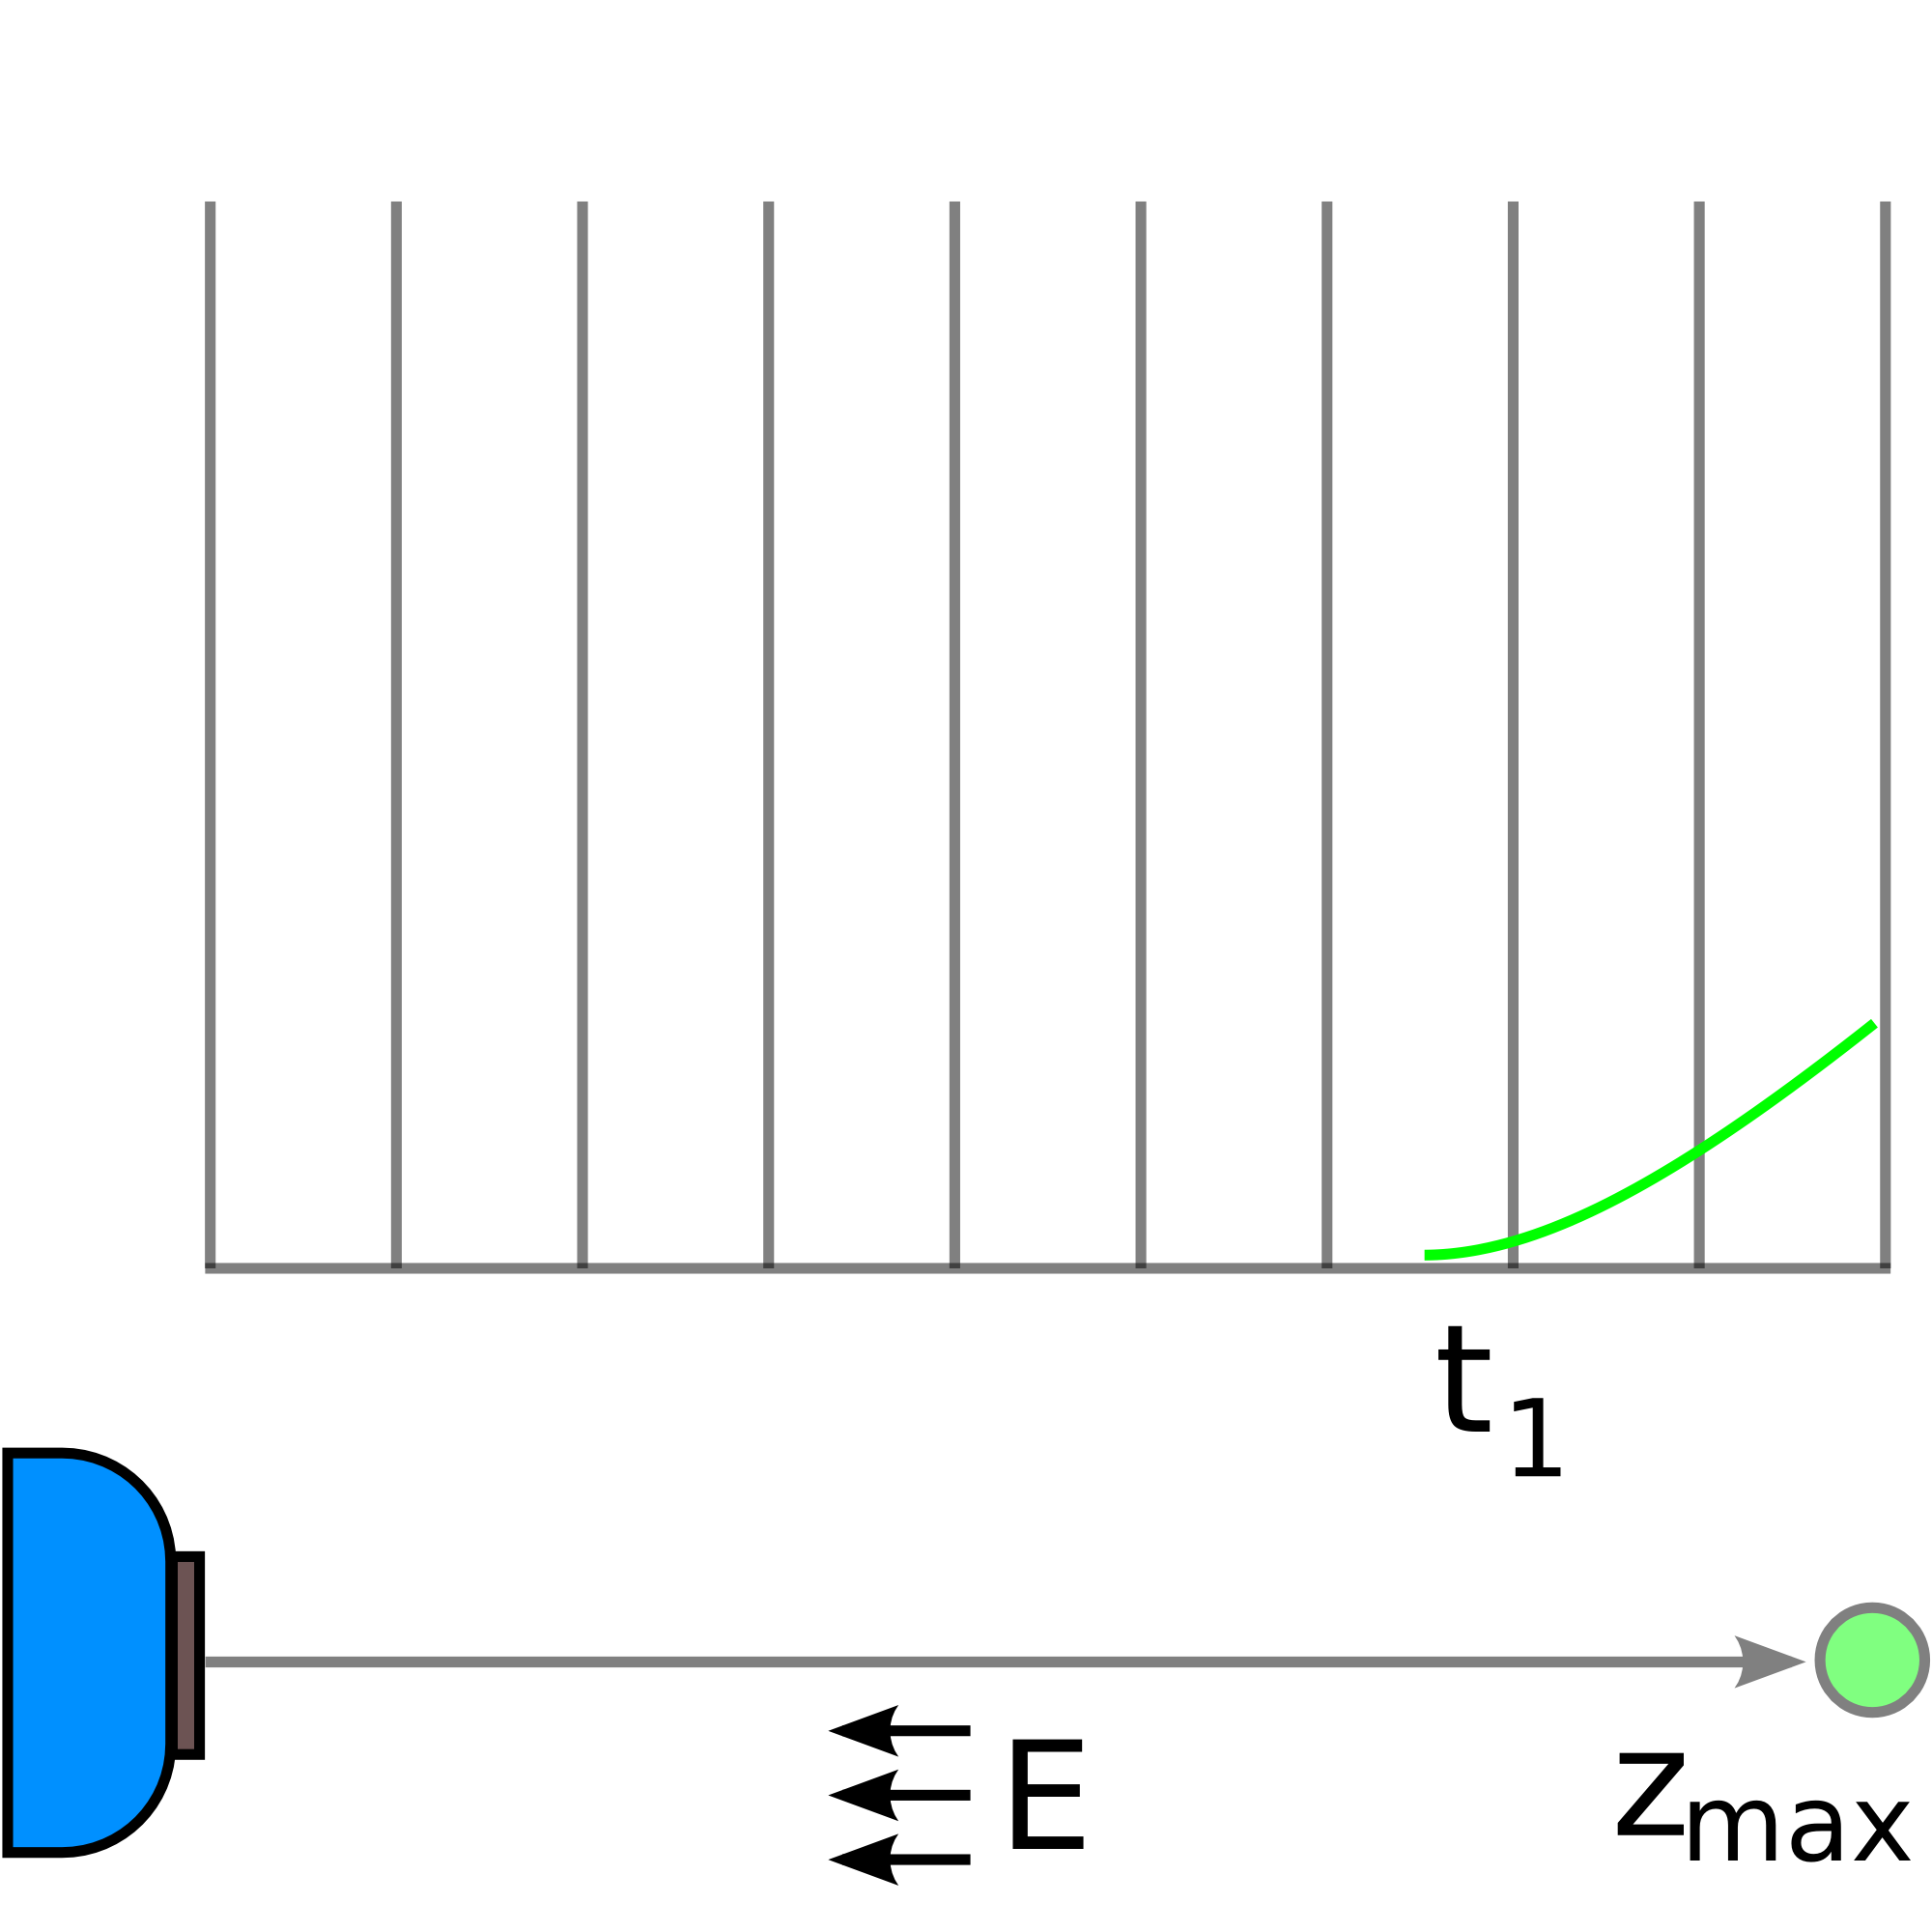
\includegraphics{bin3}}
   	    \only<4>{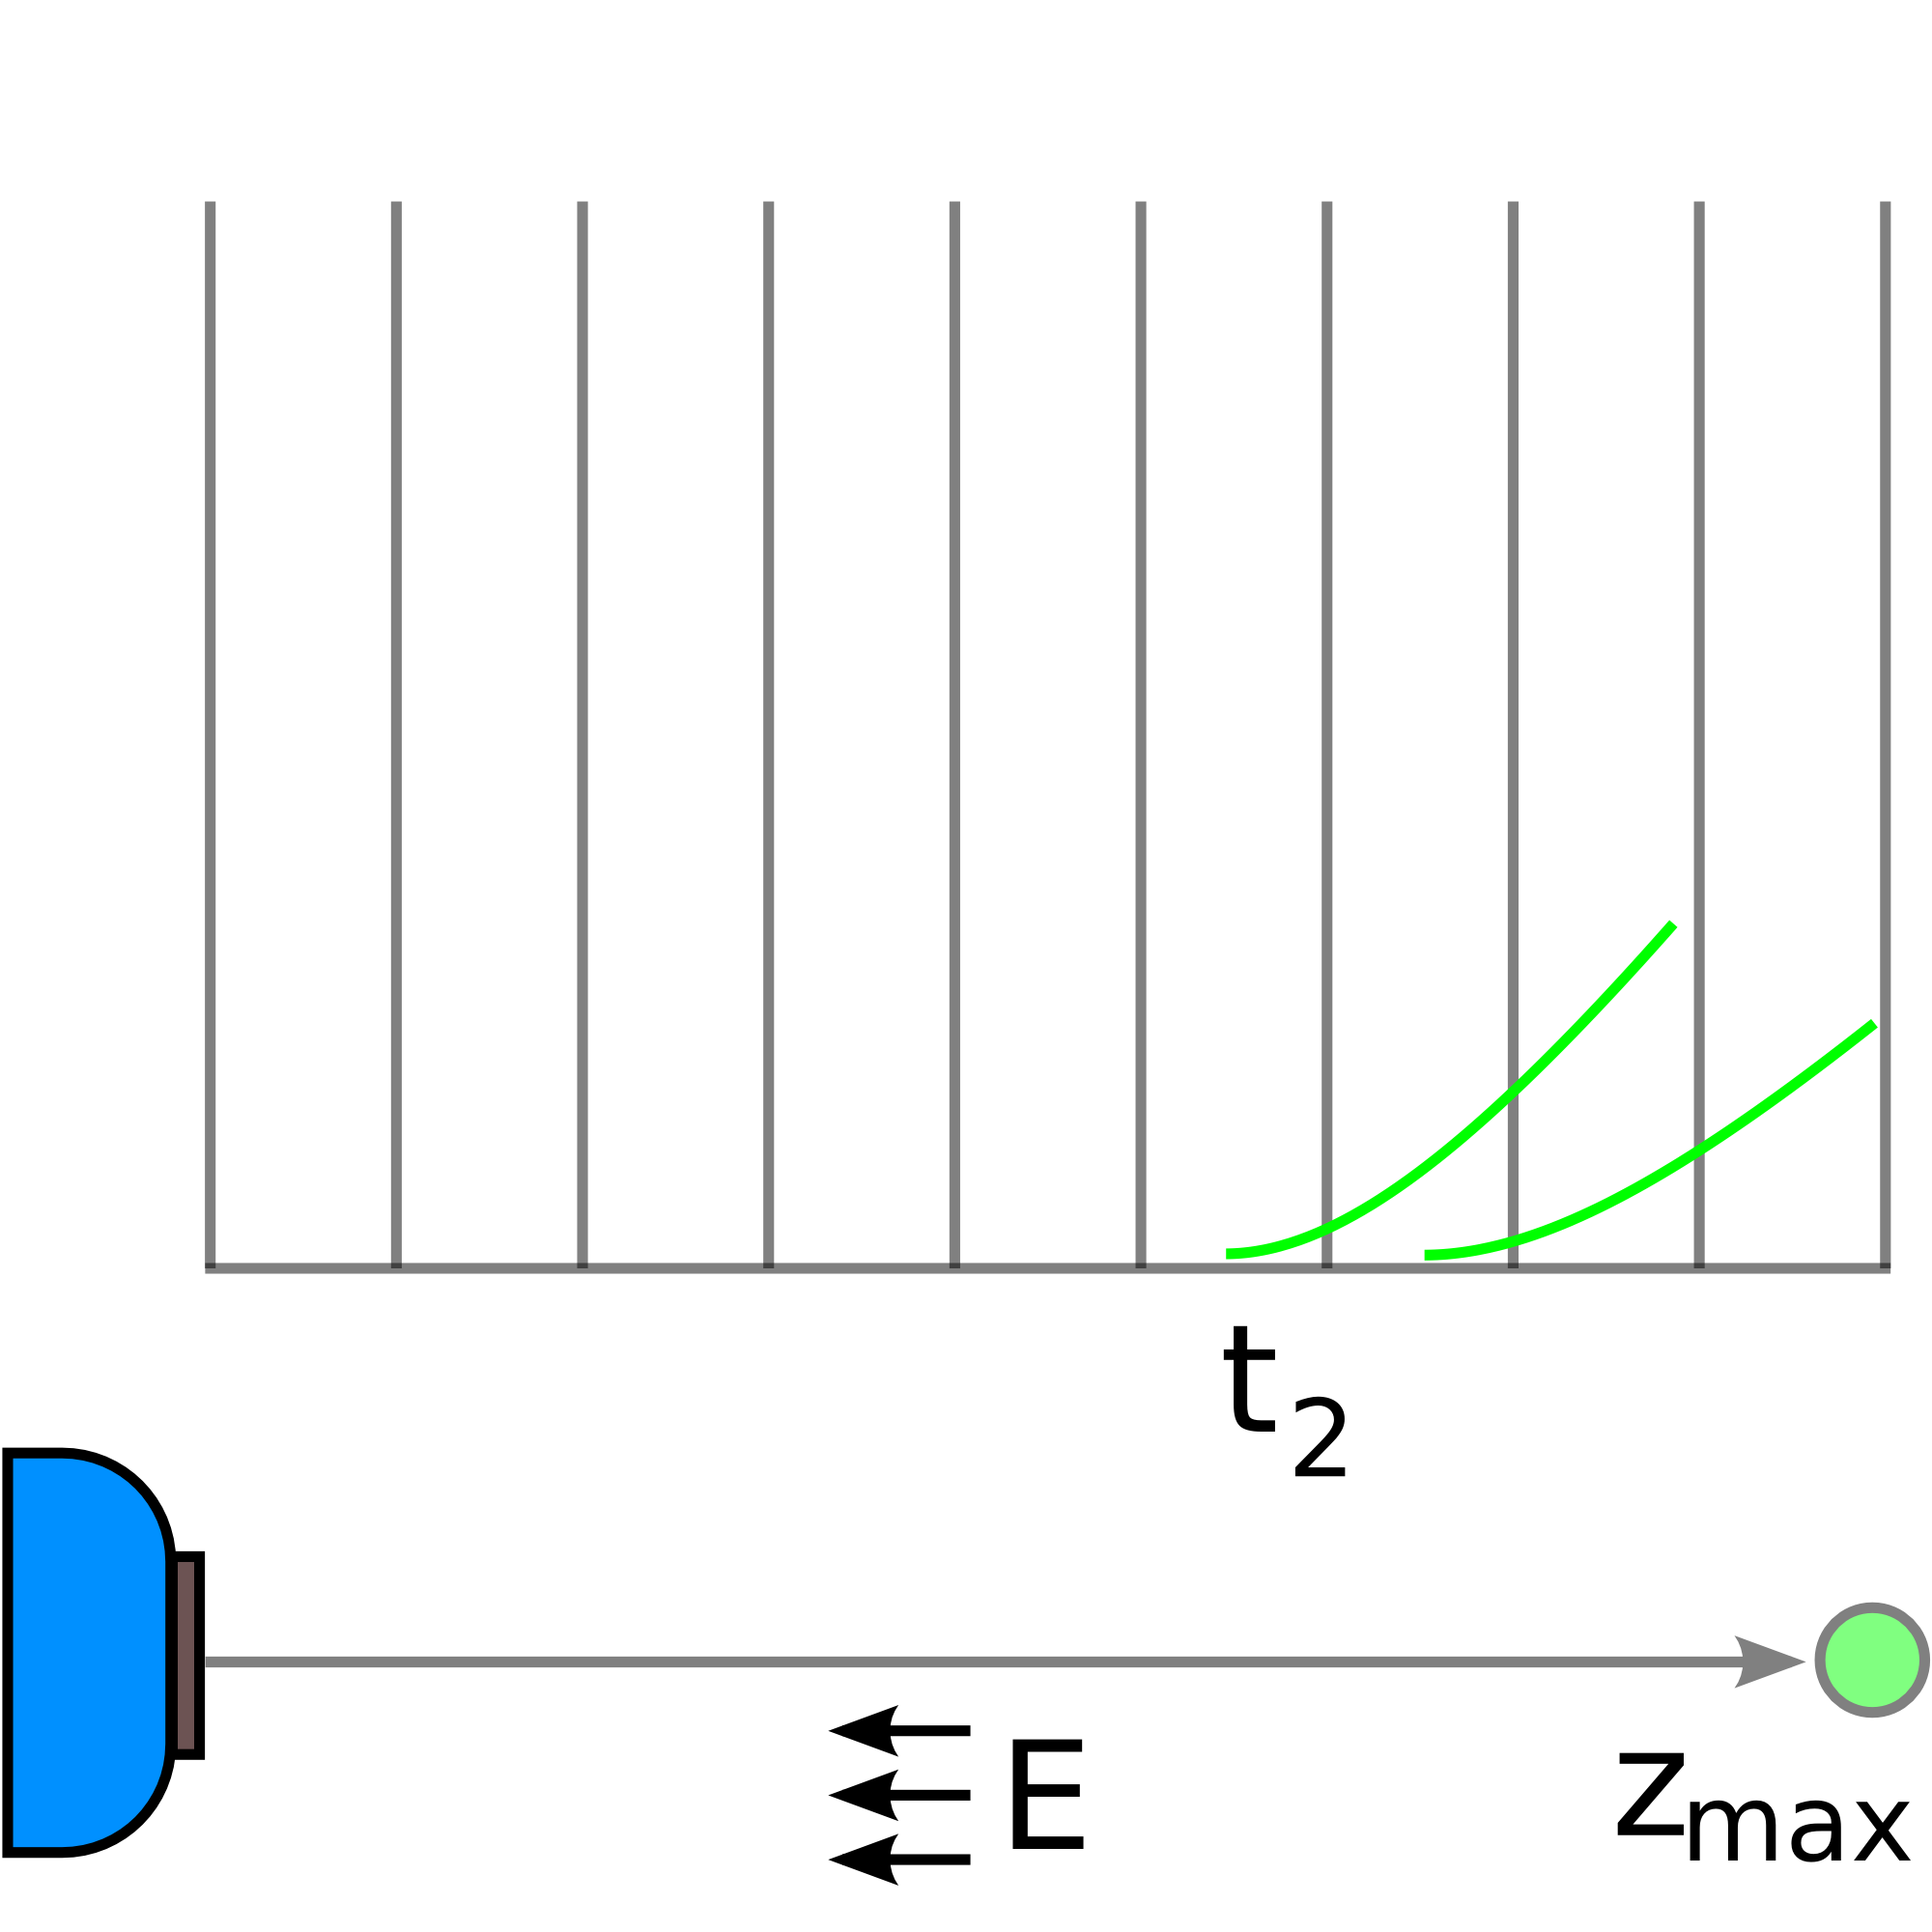
\includegraphics{bin4}}
    	\only<5>{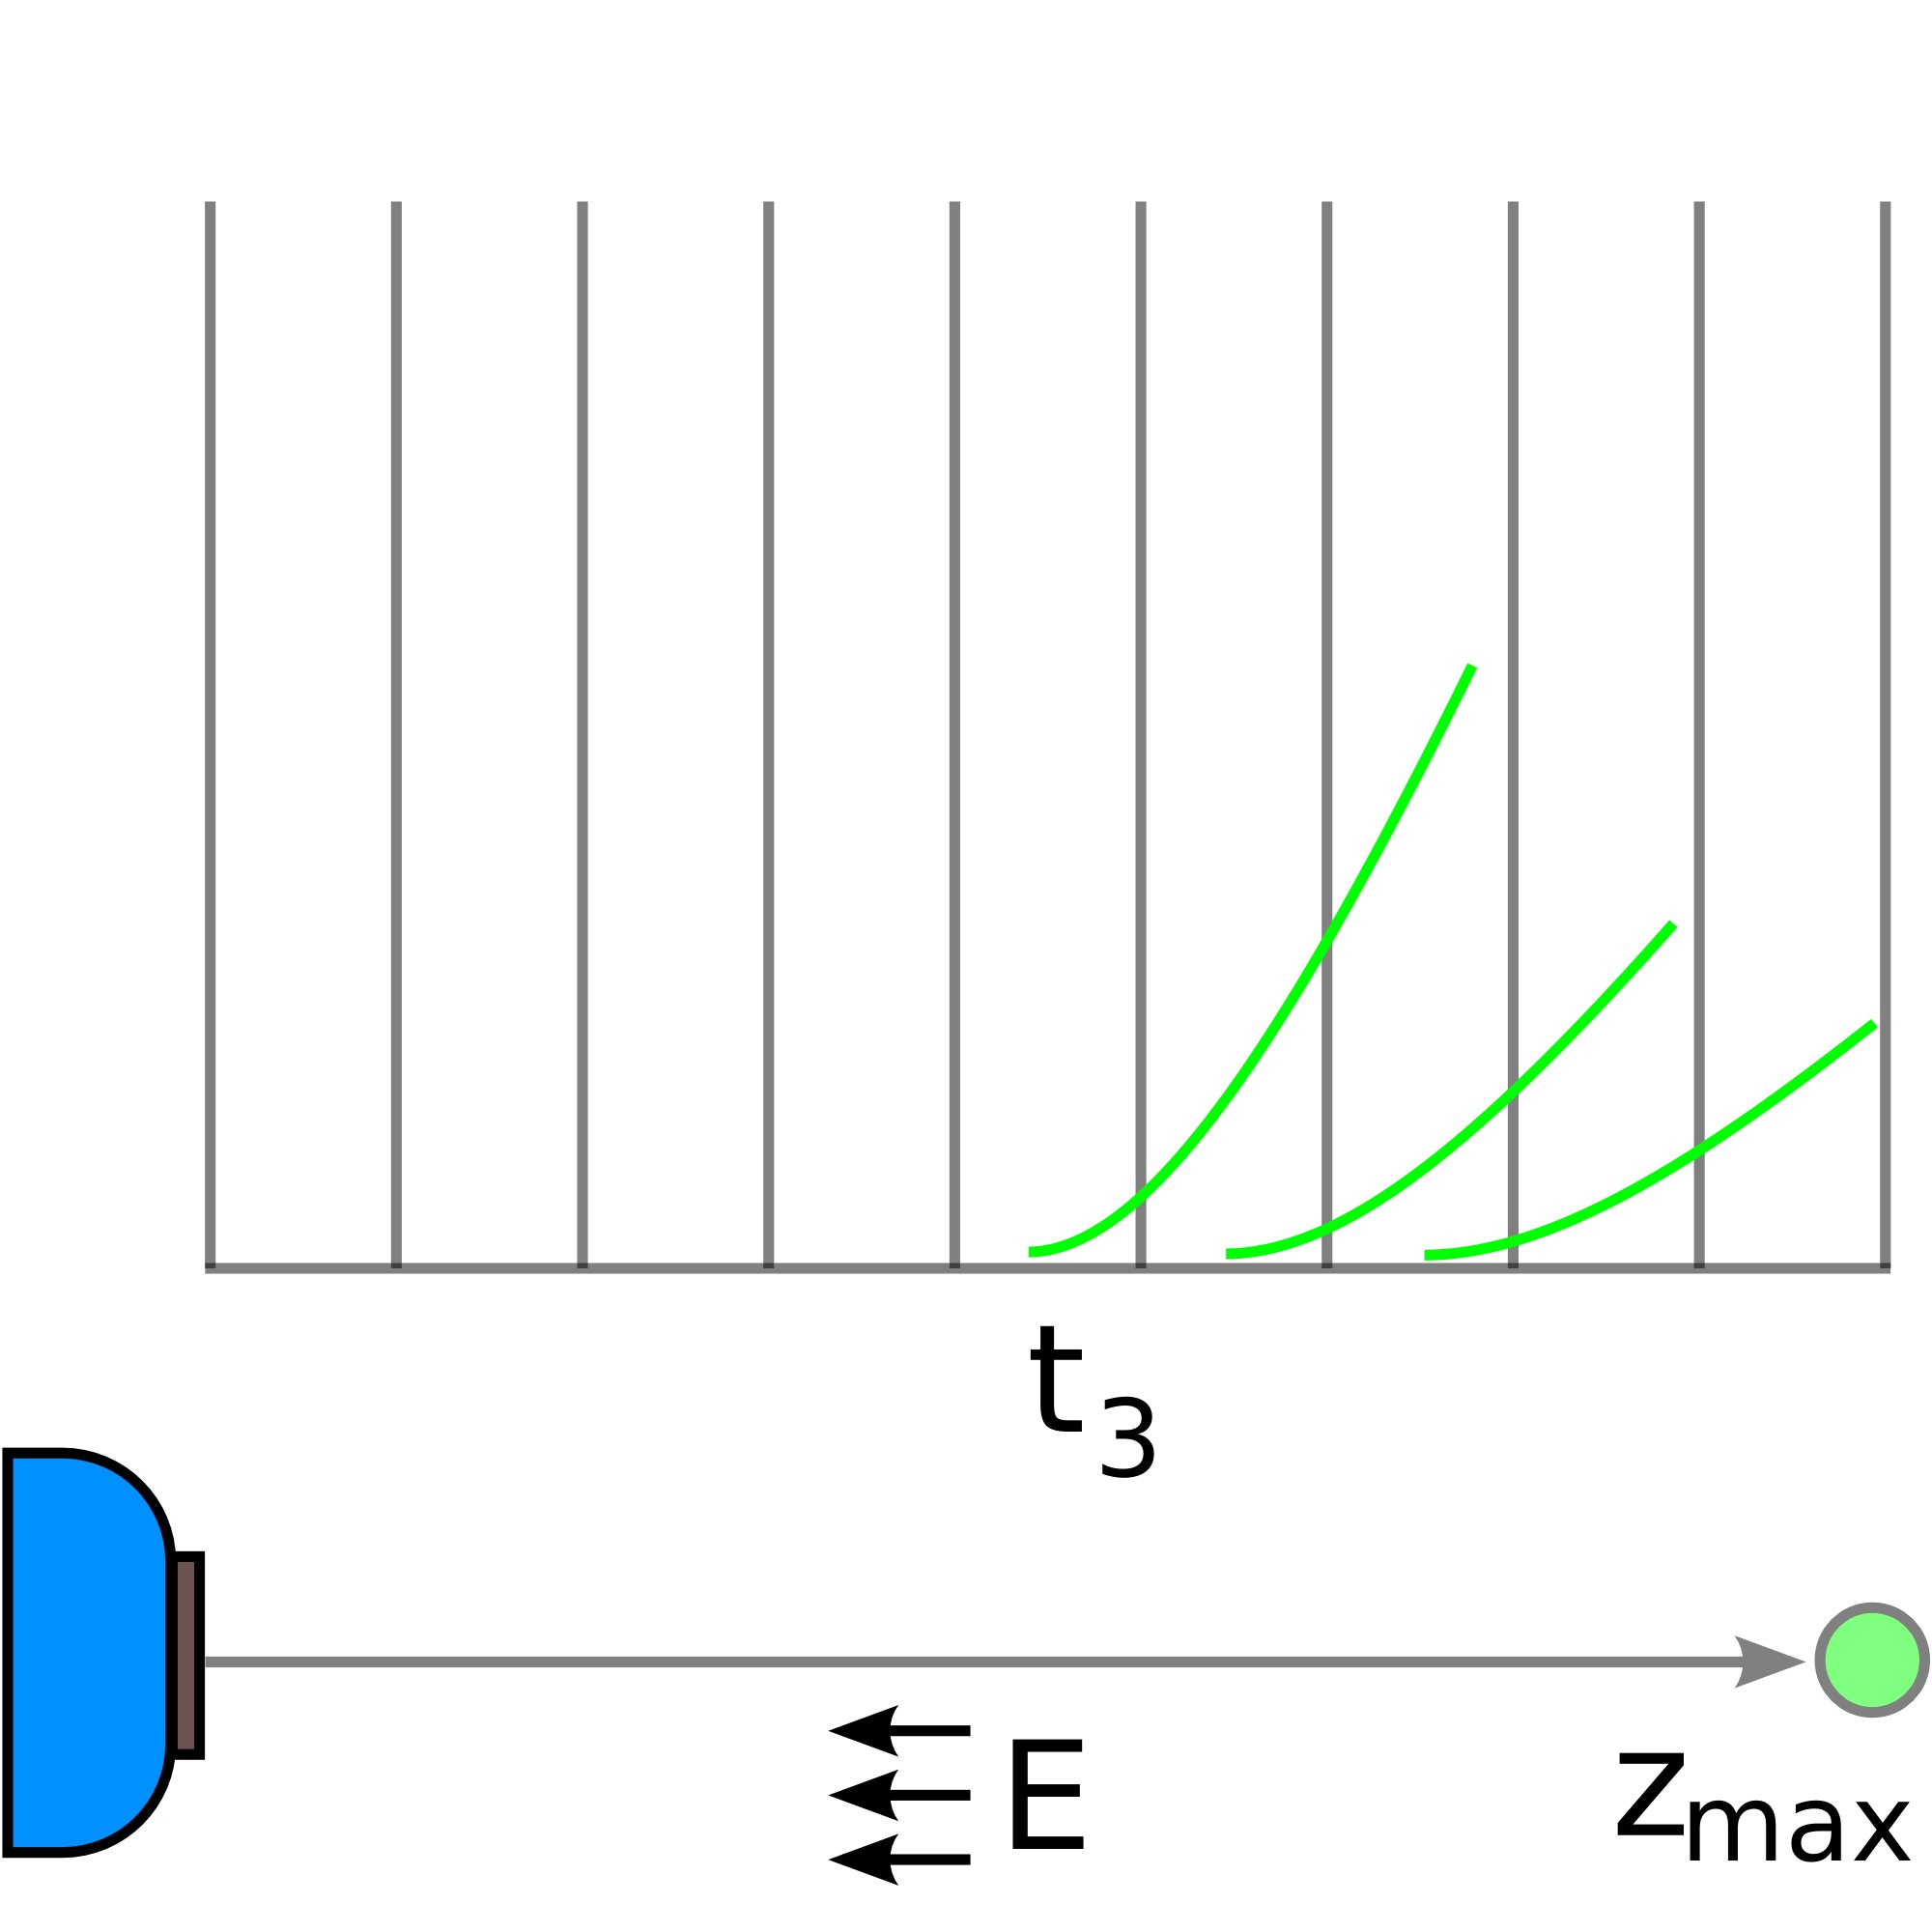
\includegraphics{bin5}}
    	\only<6>{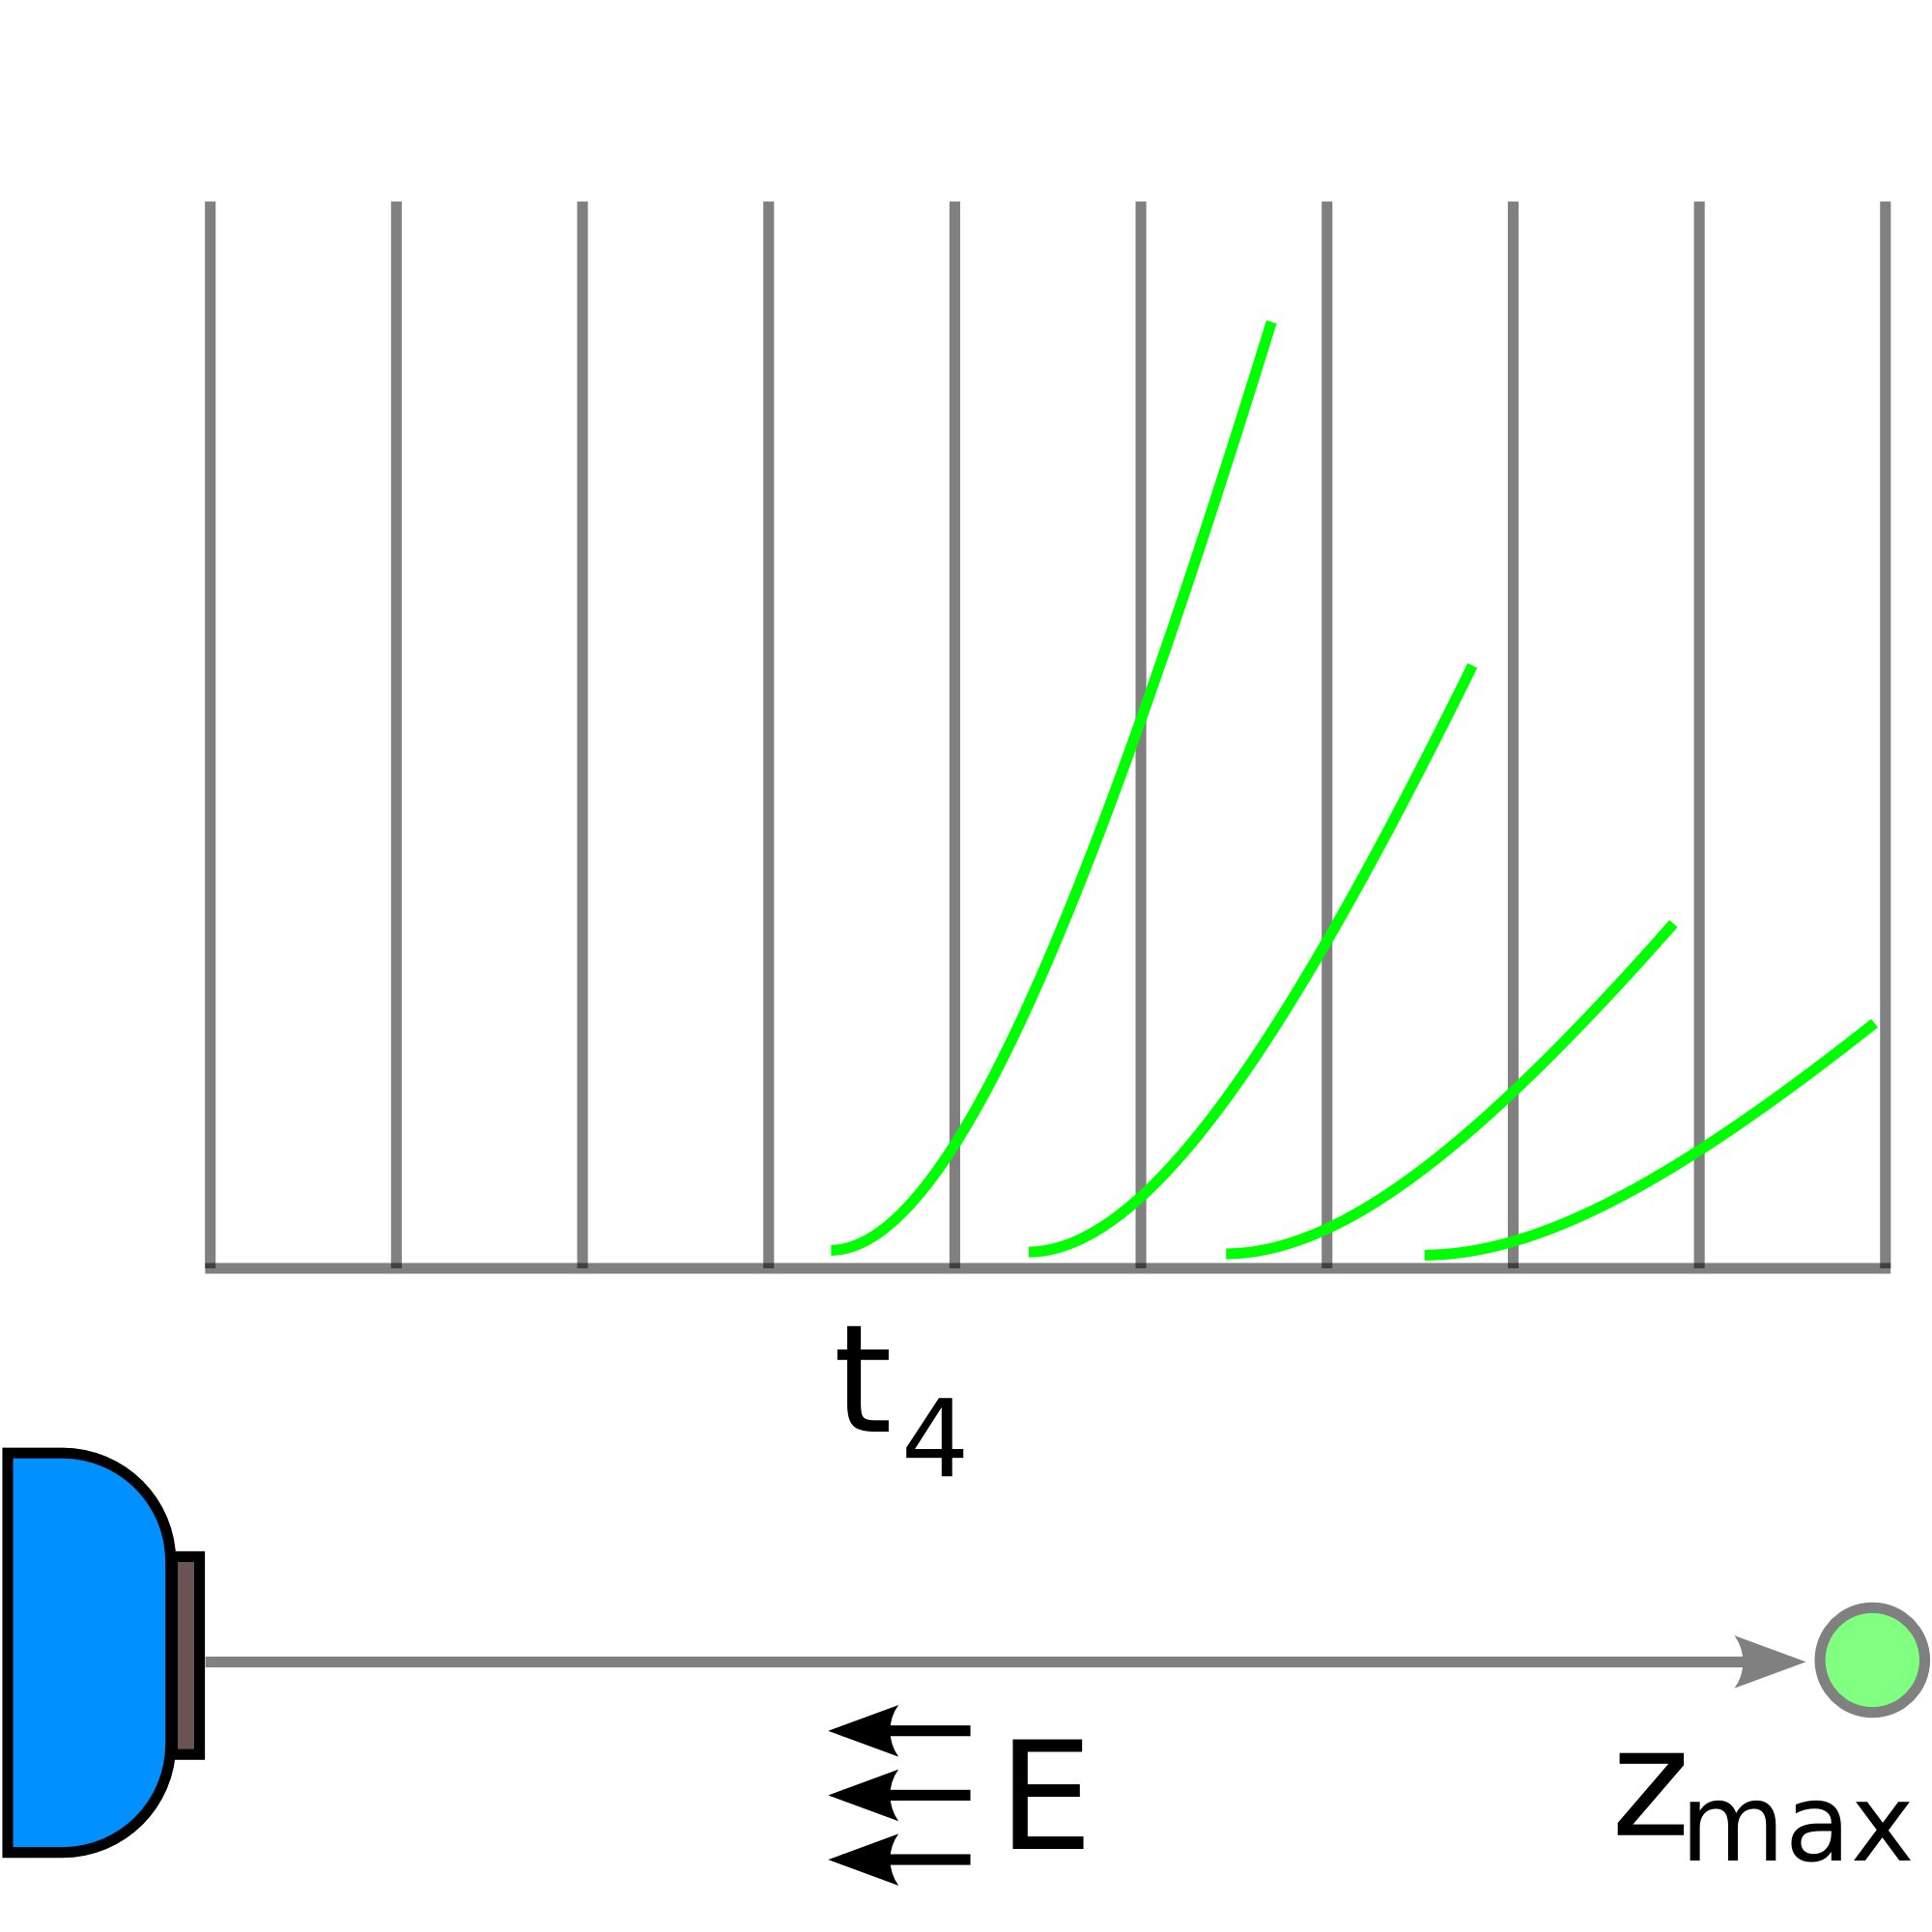
\includegraphics{bin6}}
    	\only<7>{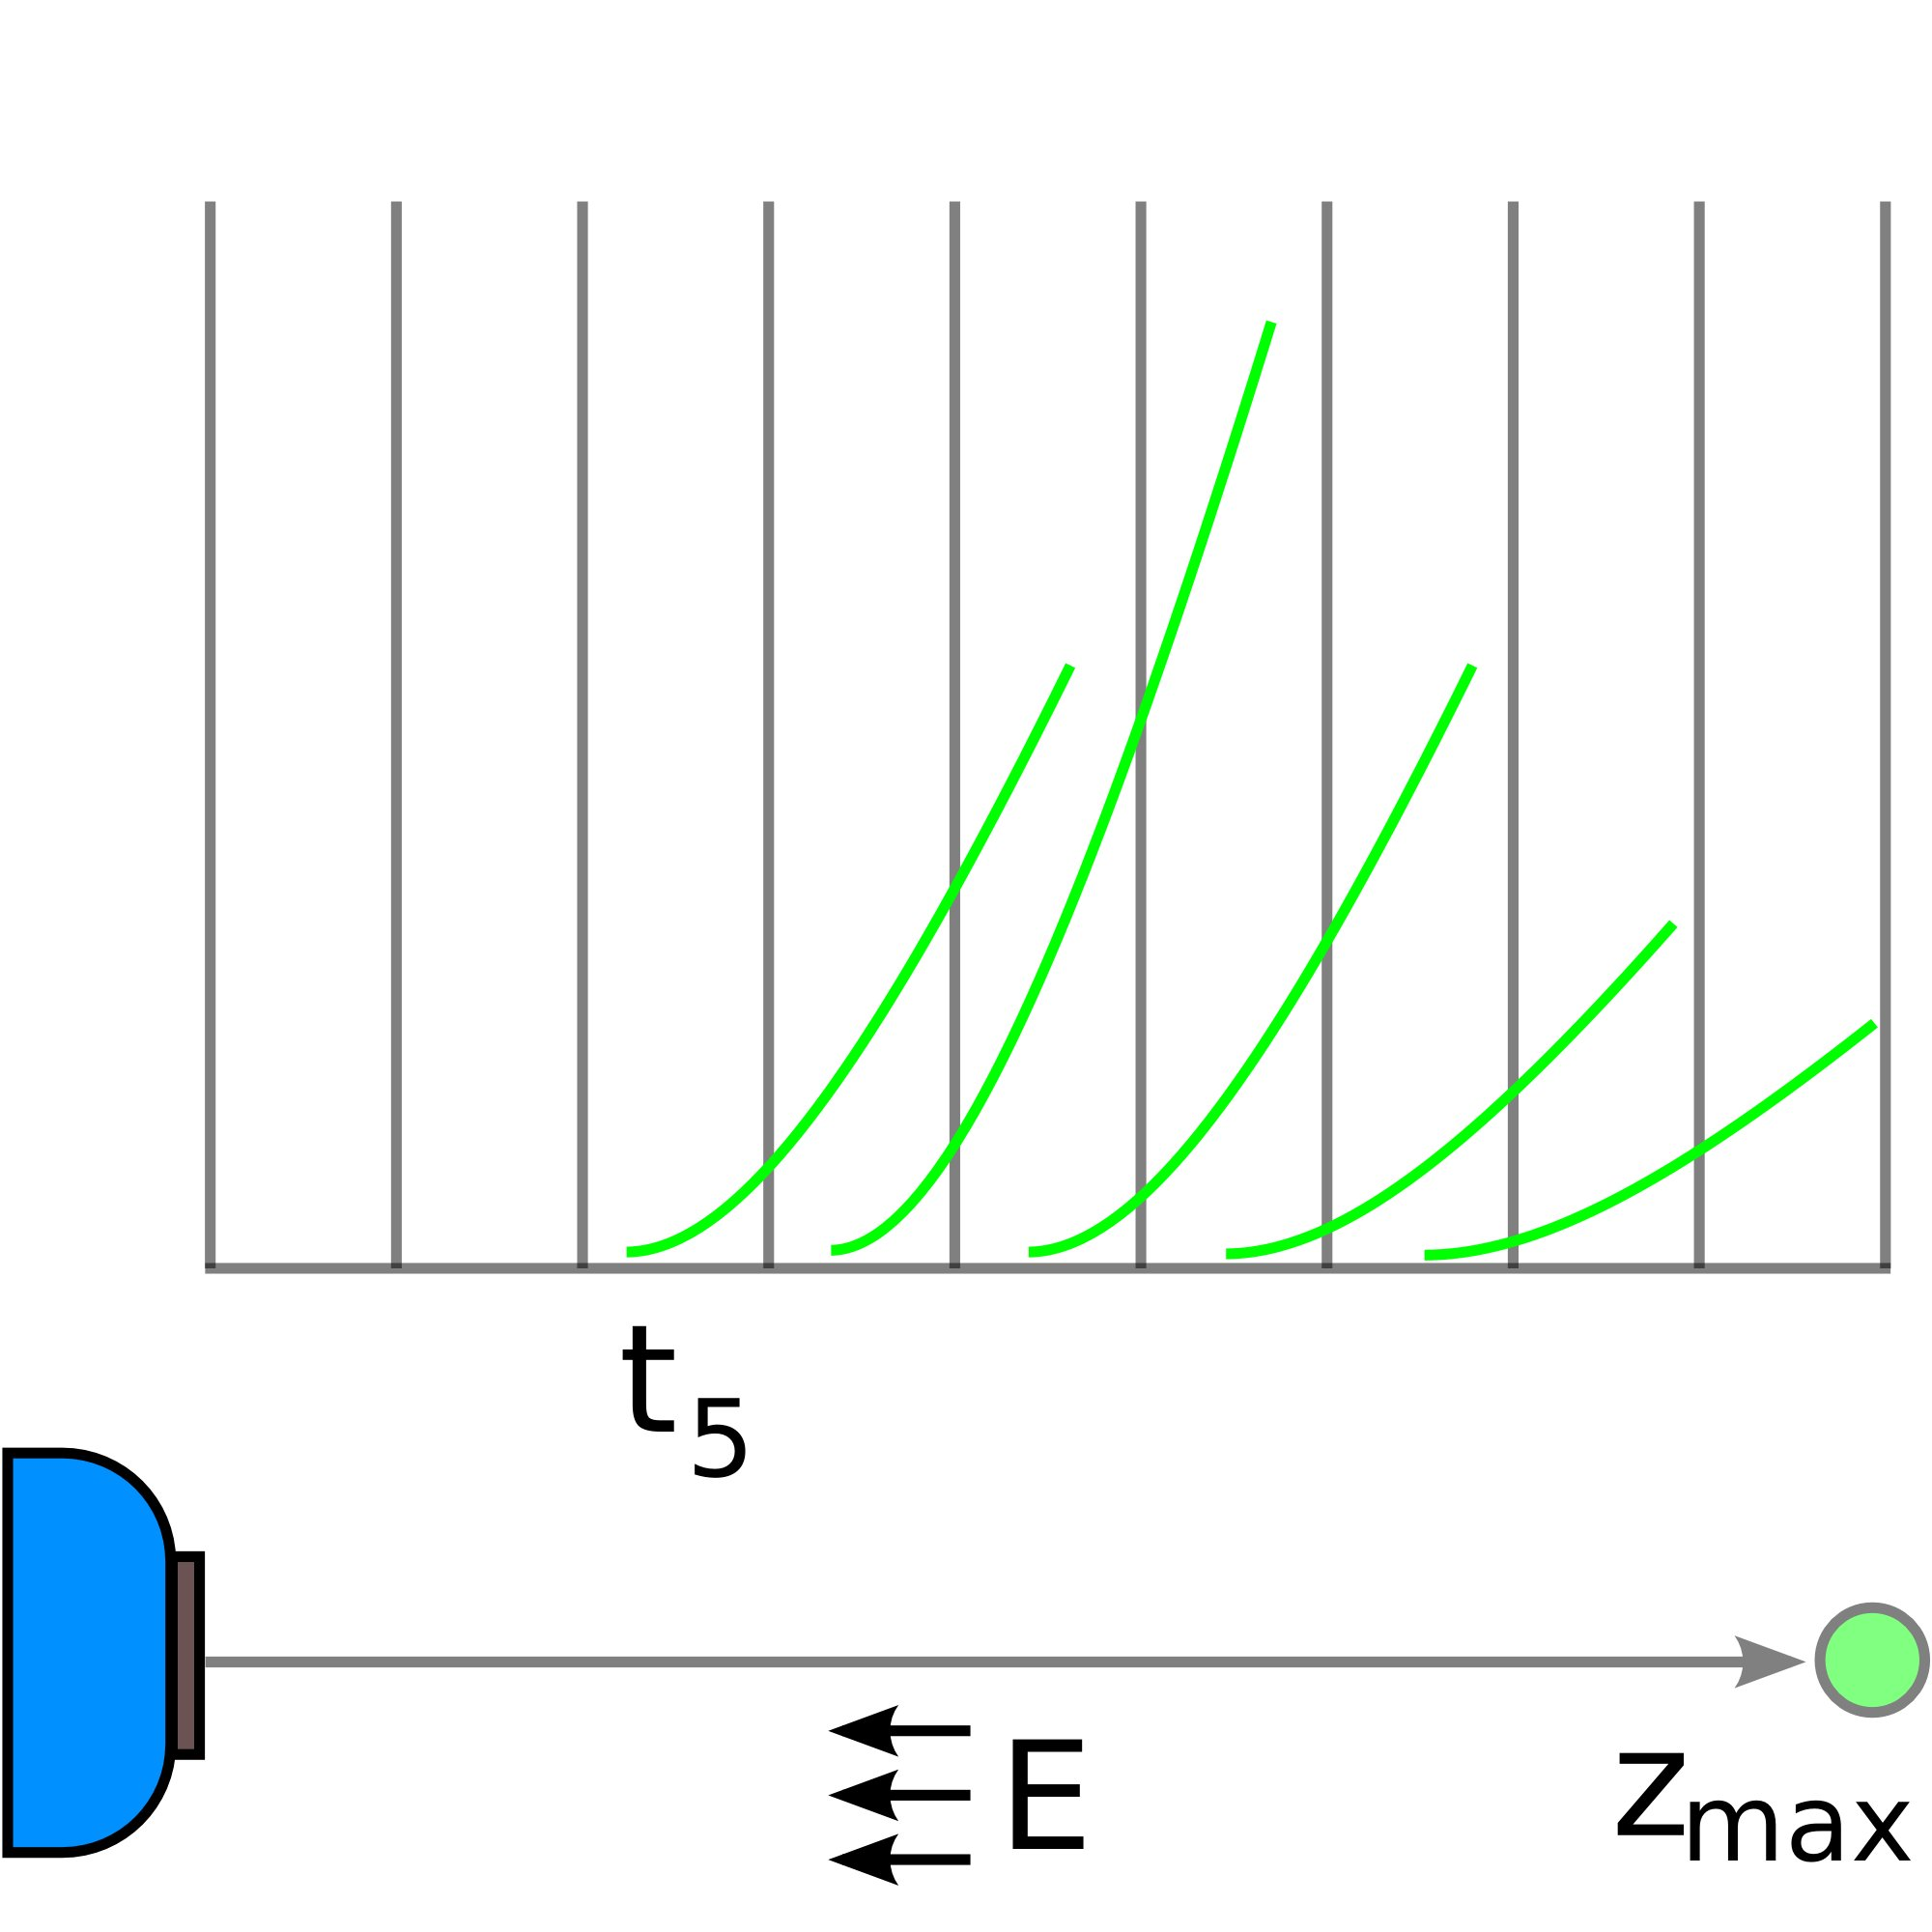
\includegraphics{bin7}}
    	\only<8>{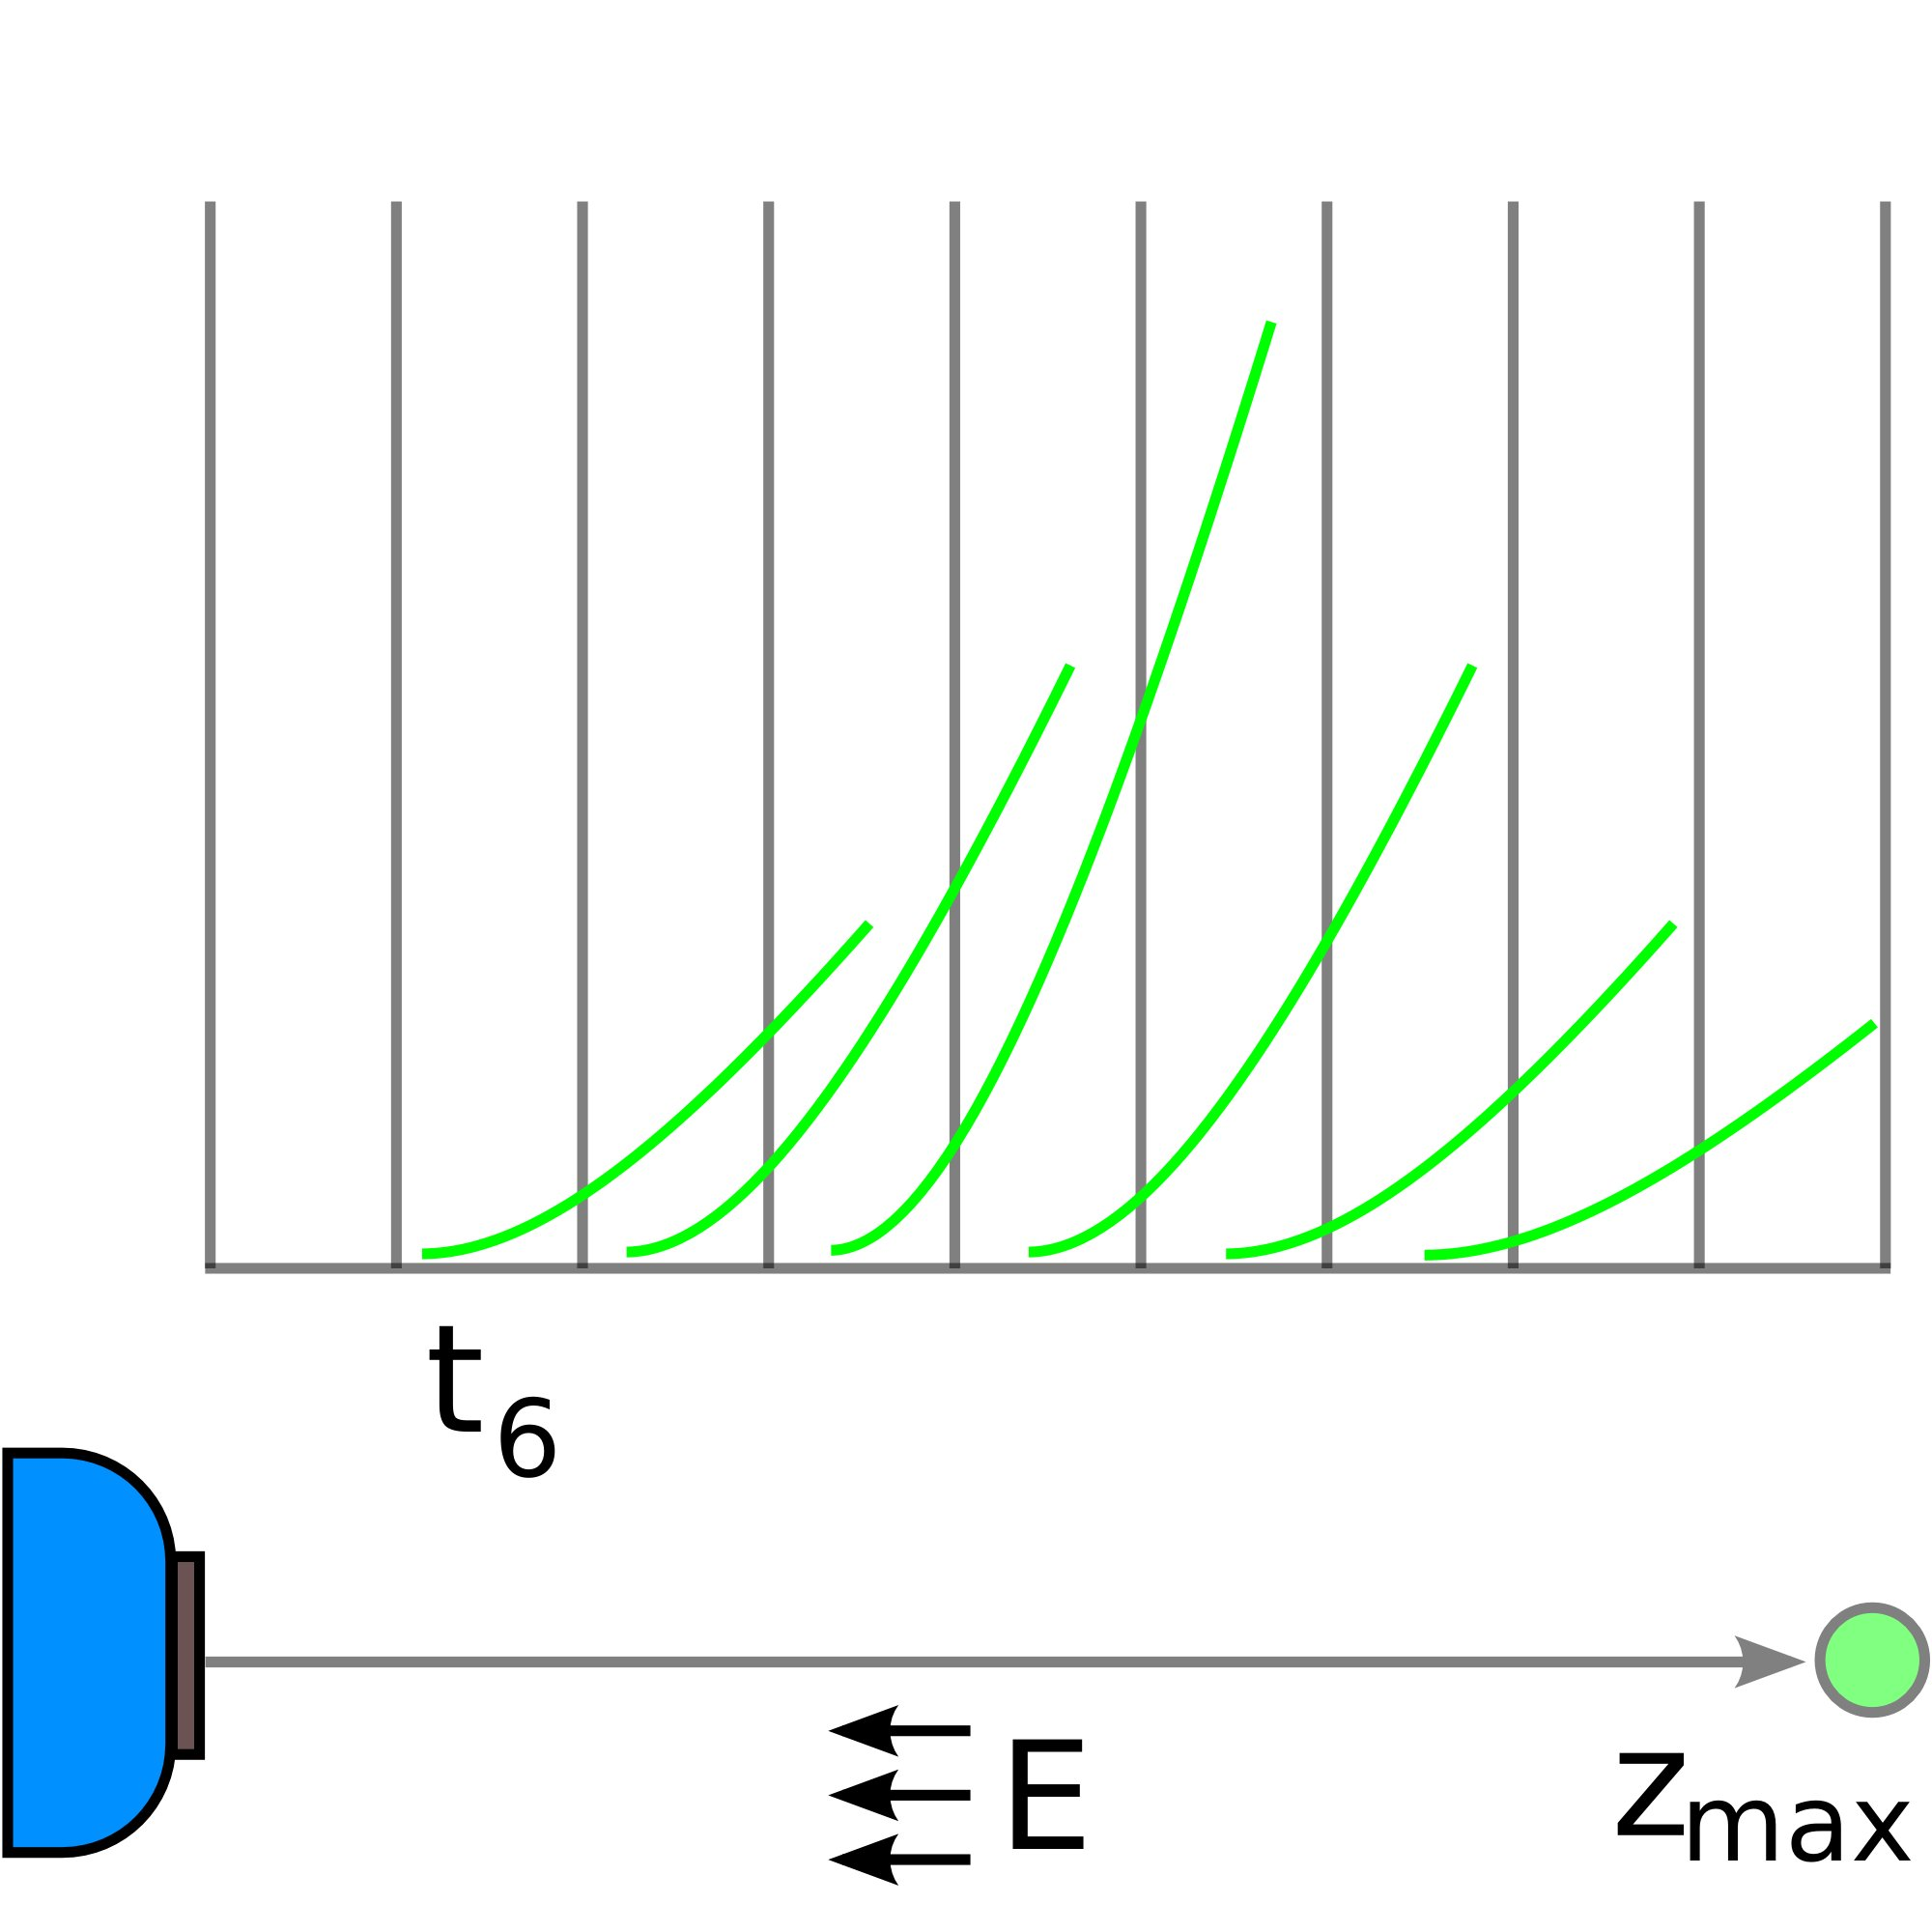
\includegraphics{bin8}}
    	}
    	\only<9->{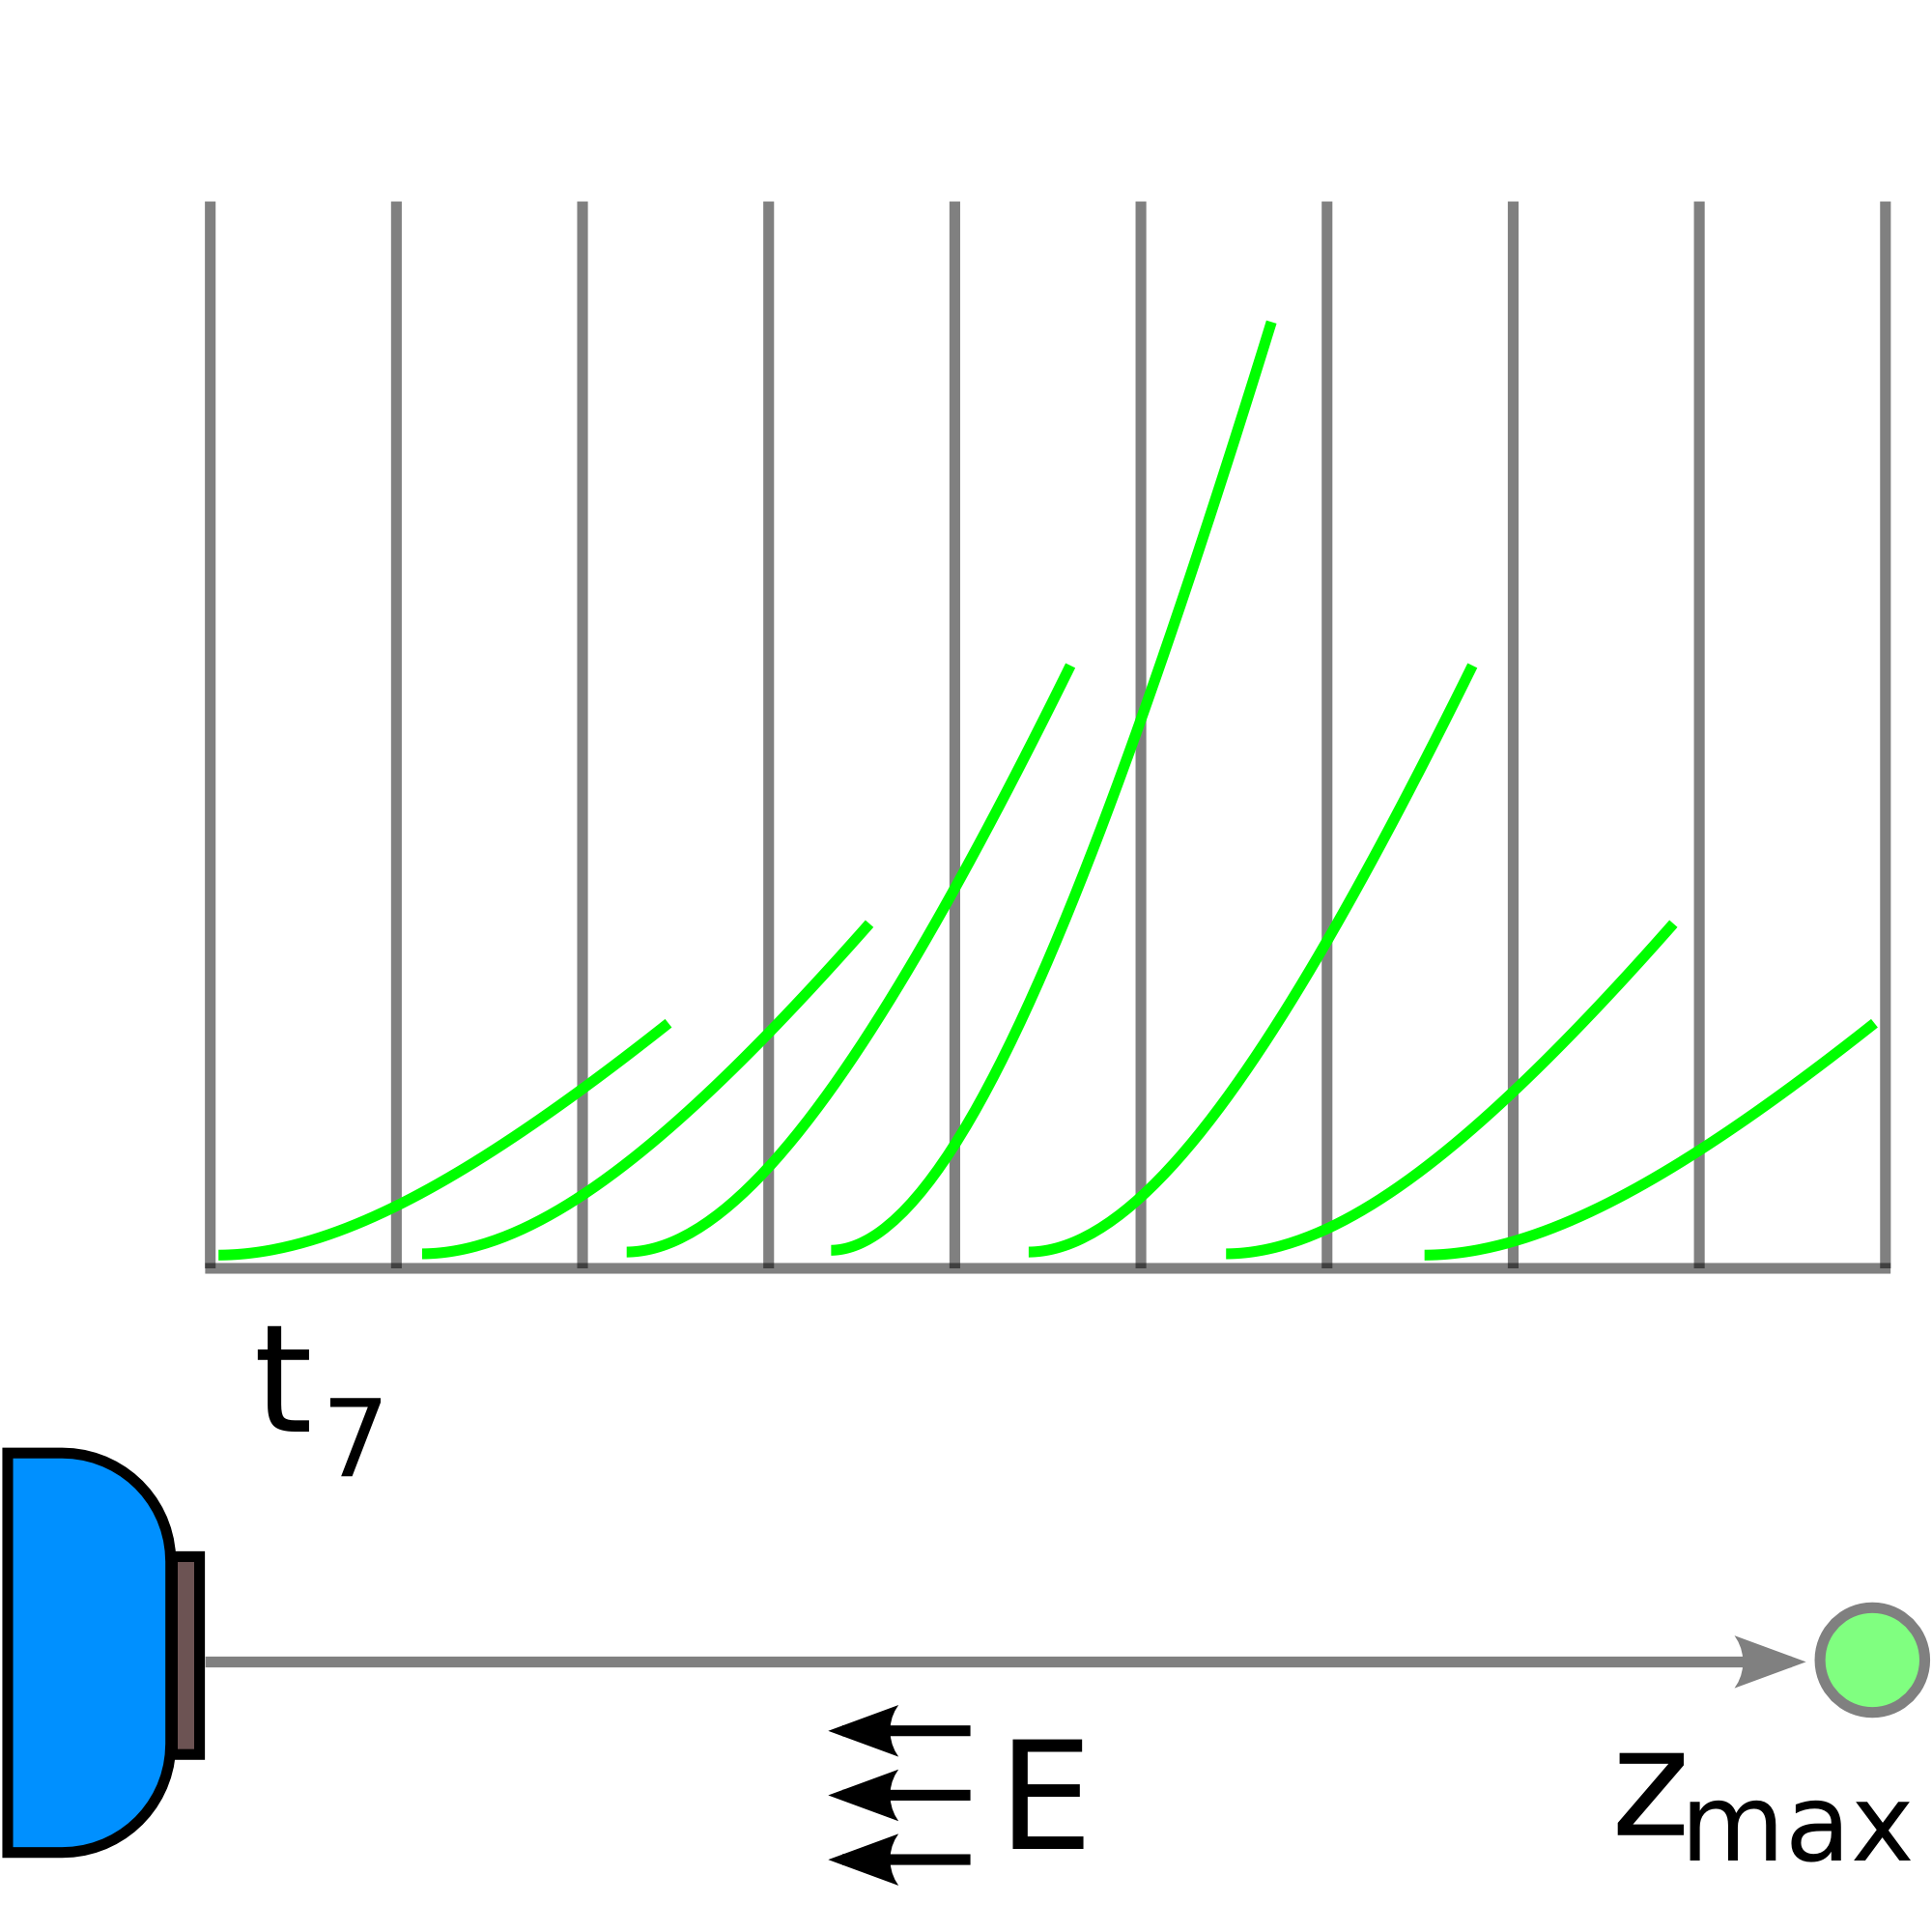
\includegraphics{bin9}}
    	\only<article>
    	{
    	\caption{Overlay of time slices of distributions of electrons in space bins}
    	}
    \end{figure}
	\end{overlayarea}
	\end{column}
\end{columns}

\end{frame}

\begin{frame}{Comparison with Sipe Model}
\begin{columns}
	\begin{column}{3in}
	\begin{figure}[H]
    	\centering
		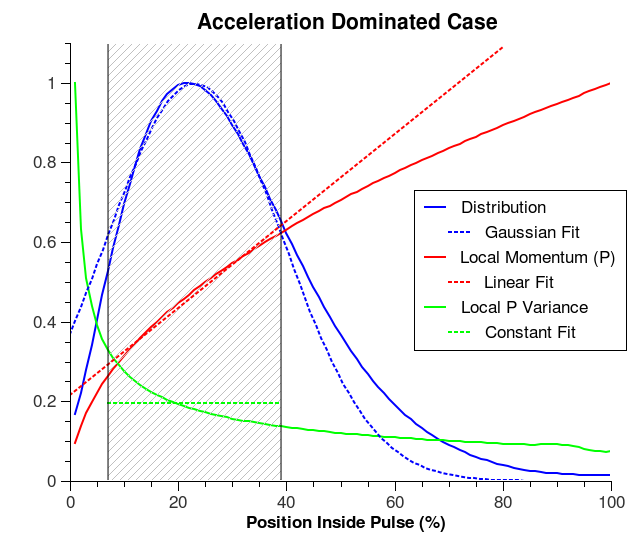
\includegraphics{Acc}
		\only<article>{\caption{Acceleration dominated case}}
	\end{figure}
	\end{column}

	\begin{column}{.38 \linewidth}
		\begin{block}{For operating conditions:}    
			$ qE/m >> v_{max}/t_{total} $
		\end{block}

		\vf
 
		\only<2->
		{
		For a majority of electrons the allowed fit is reasonable
		}

    \end{column}
\end{columns}
\end{frame}

\begin{frame}
\only<presentation>{\frametitle{Comparison with Sipe Model}}
\begin{columns}

	\begin{column}{.38 \linewidth}
		\begin{block}{For operating conditions:}    
			$ qE/m << v_{max}/t_{total} $
		\end{block}

		\vf
 
		\only<2->
		{
		In this case, the fit for ``local momentum width'' (related to
		$\eta$) not very good
		}

    \end{column}

	\begin{column}{3in}
	\begin{figure}[H]
    	\centering
		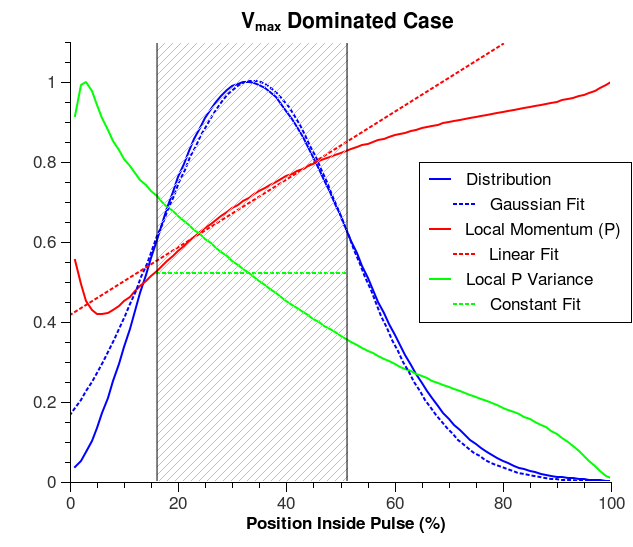
\includegraphics{Vmax}
		\only<article>{\caption{Vmax dominated case}}
	\end{figure}
	\end{column}

\end{columns}
\end{frame}

\begin{frame}
\only<presentation>{\frametitle{Comparison with Sipe Model}}
\begin{columns}
	\begin{column}{3in}
	\begin{figure}[H]
  		\centering
		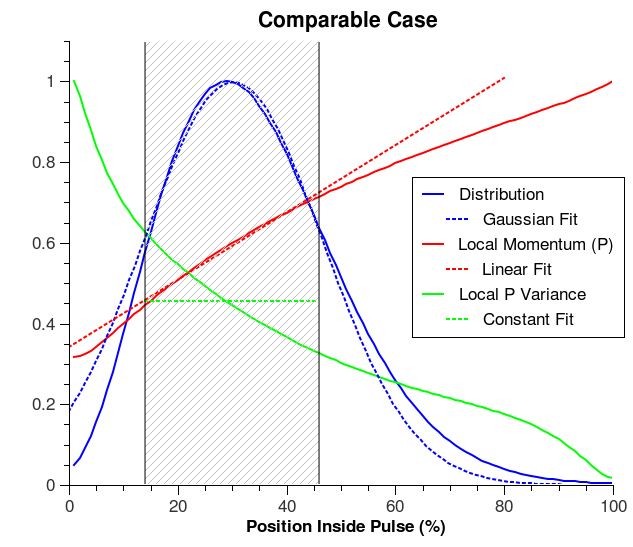
\includegraphics{Equal}
		\only<article>{\caption{Case where Vmax and Acceleration are approximately equal}}
	\end{figure}
	\end{column}

	\begin{column}{.38\linewidth}
		\begin{block}{For operating conditions:}    
			$ qE/m \approx v_{max}/t_{total} $
		\end{block}

		\vf
 
		\only<2->
		{
		Even this more intermediate case will still have some artifacts
		owing to the limitations of the model
		}

    \end{column}
\end{columns}
\end{frame}

\begin{frame}{Regenerative Laser Amplifier}
  Regenerative laser amplifier:
  \begin{columns}
    \begin{column}{0.49\linewidth}
      \begin{itemize}
        \item 650Hz
        \item 100$\mu$J fundamental
        \item<2-> [$\hookrightarrow$] Generates $10^8$ electrons
        \begin{itemize}
          \item<3-> Single-shot imaging
          \item<4-> Observe charge-charge interaction
          \item<5-> Investigate short-pulse Child's Law
        \end{itemize}
      \end{itemize}
    \end{column}
    \begin{column}{0.49\linewidth}
    \begin{center}
      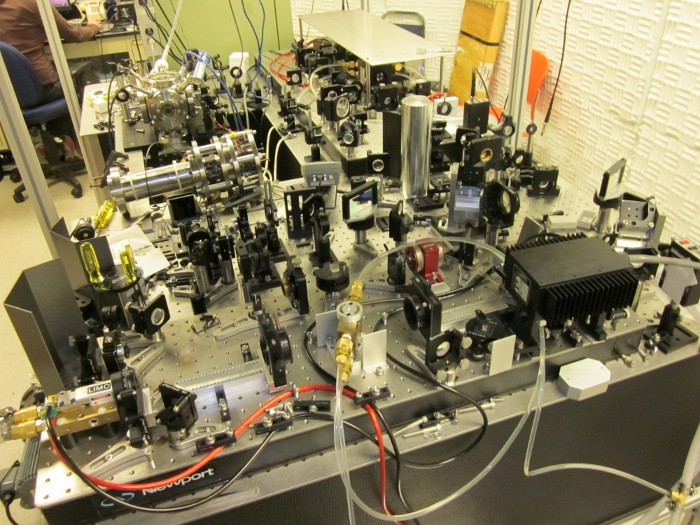
\includegraphics{regen}
    \end{center}
    \end{column}
  \end{columns}
\end{frame}

\begin{frame}{Two-photon Assisted Thermionic Emission (2PTE)}
  \begin{center}
    \begin{tikzpicture}[scale=0.8]
  %% \begin{tikzpicture}[gnuplot]
%% generated with GNUPLOT 4.6p0 (Lua 5.1; terminal rev. 99, script rev. 100)
%% Mon 08 Apr 2013 03:15:44 PM CDT
\path (0.000,0.000) rectangle (12.500,8.750);
\gpcolor{color=gp lt color border}
\gpsetlinetype{gp lt border}
\gpsetlinewidth{1.00}
\draw[gp path] (1.504,0.985)--(1.684,0.985);
\draw[gp path] (11.485,0.985)--(11.305,0.985);
\node[gp node right] at (1.320,0.985) { 0.9};
\draw[gp path] (1.504,2.042)--(1.684,2.042);
\draw[gp path] (11.485,2.042)--(11.305,2.042);
\node[gp node right] at (1.320,2.042) { 1};
\draw[gp path] (1.504,3.098)--(1.684,3.098);
\draw[gp path] (11.485,3.098)--(11.305,3.098);
\node[gp node right] at (1.320,3.098) { 1.1};
\draw[gp path] (1.504,4.155)--(1.684,4.155);
\draw[gp path] (11.485,4.155)--(11.305,4.155);
\node[gp node right] at (1.320,4.155) { 1.2};
\draw[gp path] (1.504,5.211)--(1.684,5.211);
\draw[gp path] (11.485,5.211)--(11.305,5.211);
\node[gp node right] at (1.320,5.211) { 1.3};
\draw[gp path] (1.504,6.268)--(1.684,6.268);
\draw[gp path] (11.485,6.268)--(11.305,6.268);
\node[gp node right] at (1.320,6.268) { 1.4};
\draw[gp path] (1.504,7.324)--(1.684,7.324);
\draw[gp path] (11.485,7.324)--(11.305,7.324);
\node[gp node right] at (1.320,7.324) { 1.5};
\draw[gp path] (1.504,8.381)--(1.684,8.381);
\draw[gp path] (11.485,8.381)--(11.305,8.381);
\node[gp node right] at (1.320,8.381) { 1.6};
\draw[gp path] (1.504,0.985)--(1.504,1.165);
\draw[gp path] (1.504,8.381)--(1.504,8.201);
\node[gp node center] at (1.504,0.677) { 0};
\draw[gp path] (2.920,0.985)--(2.920,1.165);
\draw[gp path] (2.920,8.381)--(2.920,8.201);
\node[gp node center] at (2.920,0.677) { 2};
\draw[gp path] (4.335,0.985)--(4.335,1.165);
\draw[gp path] (4.335,8.381)--(4.335,8.201);
\node[gp node center] at (4.335,0.677) { 4};
\draw[gp path] (5.751,0.985)--(5.751,1.165);
\draw[gp path] (5.751,8.381)--(5.751,8.201);
\node[gp node center] at (5.751,0.677) { 6};
\draw[gp path] (7.167,0.985)--(7.167,1.165);
\draw[gp path] (7.167,8.381)--(7.167,8.201);
\node[gp node center] at (7.167,0.677) { 8};
\draw[gp path] (8.583,0.985)--(8.583,1.165);
\draw[gp path] (8.583,8.381)--(8.583,8.201);
\node[gp node center] at (8.583,0.677) { 10};
\draw[gp path] (9.998,0.985)--(9.998,1.165);
\draw[gp path] (9.998,8.381)--(9.998,8.201);
\node[gp node center] at (9.998,0.677) { 12};
\draw[gp path] (11.414,0.985)--(11.414,1.165);
\draw[gp path] (11.414,8.381)--(11.414,8.201);
\node[gp node center] at (11.414,0.677) { 14};
\draw[gp path] (1.504,8.381)--(1.504,0.985)--(11.485,0.985)--(11.485,8.381)--cycle;
\node[gp node center,rotate=-270] at (0.246,4.683) {HWe$^{-1}$M Beam Size(mm)};
\node[gp node center,rotate=-270] at (11.792,4.683) {Electron Yield (a.u.)};
\node[gp node center] at (6.494,0.215) {Incident Laser Pulse Energy (nJ)};
\gpcolor{color=gp lt color 0}
\gpsetlinetype{gp lt plot 0}
\draw[gp path] (1.504,1.217)--(2.495,2.063)--(3.486,2.718)--(4.477,3.267)--(5.468,3.732)%
  --(6.459,4.155)--(7.450,4.535)--(8.441,4.873)--(9.432,5.190)--(10.423,5.465)--(11.414,5.761);
\gpcolor{rgb color={1.000,0.000,0.000}}
\gpsetlinetype{gp lt plot 1}
\draw[gp path] (1.504,1.196)--(2.495,2.232)--(3.486,2.992)--(4.477,3.605)--(5.468,4.134)%
  --(6.459,4.577)--(7.450,5.000)--(8.441,5.359)--(9.432,5.718)--(10.423,6.035)--(11.414,6.331);
\draw[gp path] (1.504,1.260)--(2.495,1.999)--(3.486,2.570)--(4.477,3.035)--(5.468,3.457)%
  --(6.459,3.838)--(7.450,4.176)--(8.441,4.493)--(9.432,4.768)--(10.423,5.042)--(11.414,5.296);
\gpcolor{rgb color={0.000,0.000,0.000}}
\gpsetlinetype{gp lt plot 4}
\draw[gp path] (3.688,1.264)--(3.688,4.008);
\draw[gp path] (3.598,1.264)--(3.778,1.264);
\draw[gp path] (3.598,4.008)--(3.778,4.008);
\draw[gp path] (4.287,2.116)--(4.287,3.716);
\draw[gp path] (4.197,2.116)--(4.377,2.116);
\draw[gp path] (4.197,3.716)--(4.377,3.716);
\draw[gp path] (4.928,2.538)--(4.928,4.890);
\draw[gp path] (4.838,2.538)--(5.018,2.538);
\draw[gp path] (4.838,4.890)--(5.018,4.890);
\draw[gp path] (5.599,2.493)--(5.599,5.320);
\draw[gp path] (5.509,2.493)--(5.689,2.493);
\draw[gp path] (5.509,5.320)--(5.689,5.320);
\draw[gp path] (6.286,2.760)--(6.286,5.543);
\draw[gp path] (6.196,2.760)--(6.376,2.760);
\draw[gp path] (6.196,5.543)--(6.376,5.543);
\draw[gp path] (6.977,3.202)--(6.977,5.528);
\draw[gp path] (6.887,3.202)--(7.067,3.202);
\draw[gp path] (6.887,5.528)--(7.067,5.528);
\draw[gp path] (7.658,3.602)--(7.658,6.057);
\draw[gp path] (7.568,3.602)--(7.748,3.602);
\draw[gp path] (7.568,6.057)--(7.748,6.057);
\draw[gp path] (8.315,3.977)--(8.315,6.160);
\draw[gp path] (8.225,3.977)--(8.405,3.977);
\draw[gp path] (8.225,6.160)--(8.405,6.160);
\draw[gp path] (8.937,3.952)--(8.937,6.196);
\draw[gp path] (8.847,3.952)--(9.027,3.952);
\draw[gp path] (8.847,6.196)--(9.027,6.196);
\draw[gp path] (9.510,4.271)--(9.510,6.210);
\draw[gp path] (9.420,4.271)--(9.600,4.271);
\draw[gp path] (9.420,6.210)--(9.600,6.210);
\draw[gp path] (10.024,4.232)--(10.024,6.801);
\draw[gp path] (9.934,4.232)--(10.114,4.232);
\draw[gp path] (9.934,6.801)--(10.114,6.801);
\draw[gp path] (10.468,4.526)--(10.468,6.879);
\draw[gp path] (10.378,4.526)--(10.558,4.526);
\draw[gp path] (10.378,6.879)--(10.558,6.879);
\draw[gp path] (10.834,4.756)--(10.834,7.107);
\draw[gp path] (10.744,4.756)--(10.924,4.756);
\draw[gp path] (10.744,7.107)--(10.924,7.107);
\draw[gp path] (11.115,4.773)--(11.115,7.151);
\draw[gp path] (11.025,4.773)--(11.205,4.773);
\draw[gp path] (11.025,7.151)--(11.205,7.151);
\draw[gp path] (11.306,5.090)--(11.306,7.068);
\draw[gp path] (11.216,5.090)--(11.396,5.090);
\draw[gp path] (11.216,7.068)--(11.396,7.068);
\draw[gp path] (11.402,4.990)--(11.402,7.493);
\draw[gp path] (11.312,4.990)--(11.492,4.990);
\draw[gp path] (11.312,7.493)--(11.492,7.493);
\gpsetpointsize{4.00}
\gppoint{gp mark 5}{(3.688,2.636)}
\gppoint{gp mark 5}{(4.287,2.916)}
\gppoint{gp mark 5}{(4.928,3.714)}
\gppoint{gp mark 5}{(5.599,3.907)}
\gppoint{gp mark 5}{(6.286,4.152)}
\gppoint{gp mark 5}{(6.977,4.365)}
\gppoint{gp mark 5}{(7.658,4.830)}
\gppoint{gp mark 5}{(8.315,5.068)}
\gppoint{gp mark 5}{(8.937,5.074)}
\gppoint{gp mark 5}{(9.510,5.240)}
\gppoint{gp mark 5}{(10.024,5.516)}
\gppoint{gp mark 5}{(10.468,5.703)}
\gppoint{gp mark 5}{(10.834,5.932)}
\gppoint{gp mark 5}{(11.115,5.962)}
\gppoint{gp mark 5}{(11.306,6.079)}
\gppoint{gp mark 5}{(11.402,6.242)}
\gpcolor{rgb color={0.000,1.000,0.000}}
\gpsetlinetype{gp lt plot 0}
\draw[gp path] (2.966,0.985)--(3.016,0.988)--(3.117,0.995)--(3.218,1.002)--(3.319,1.011)%
  --(3.420,1.020)--(3.520,1.030)--(3.621,1.040)--(3.722,1.052)--(3.823,1.065)--(3.924,1.078)%
  --(4.024,1.092)--(4.125,1.107)--(4.226,1.122)--(4.327,1.139)--(4.428,1.156)--(4.529,1.174)%
  --(4.629,1.193)--(4.730,1.213)--(4.831,1.233)--(4.932,1.255)--(5.033,1.277)--(5.133,1.300)%
  --(5.234,1.324)--(5.335,1.349)--(5.436,1.374)--(5.537,1.400)--(5.638,1.427)--(5.738,1.455)%
  --(5.839,1.484)--(5.940,1.513)--(6.041,1.544)--(6.142,1.575)--(6.242,1.607)--(6.343,1.640)%
  --(6.444,1.673)--(6.545,1.708)--(6.646,1.743)--(6.747,1.779)--(6.847,1.816)--(6.948,1.854)%
  --(7.049,1.892)--(7.150,1.931)--(7.251,1.971)--(7.351,2.012)--(7.452,2.054)--(7.553,2.097)%
  --(7.654,2.140)--(7.755,2.184)--(7.856,2.229)--(7.956,2.275)--(8.057,2.322)--(8.158,2.369)%
  --(8.259,2.417)--(8.360,2.467)--(8.460,2.516)--(8.561,2.567)--(8.662,2.619)--(8.763,2.671)%
  --(8.864,2.724)--(8.965,2.778)--(9.065,2.833)--(9.166,2.889)--(9.267,2.945)--(9.368,3.002)%
  --(9.469,3.060)--(9.569,3.119)--(9.670,3.179)--(9.771,3.239)--(9.872,3.300)--(9.973,3.363)%
  --(10.074,3.426)--(10.174,3.489)--(10.275,3.554)--(10.376,3.619)--(10.477,3.685)--(10.578,3.752)%
  --(10.678,3.820)--(10.779,3.889)--(10.880,3.958)--(10.981,4.029)--(11.082,4.100)--(11.183,4.172)%
  --(11.283,4.244)--(11.384,4.318)--(11.485,4.392);
\gpcolor{rgb color={0.000,0.000,0.000}}
\gppoint{gp mark 7}{(2.895,0.997)}
\gppoint{gp mark 7}{(3.143,0.985)}
\gppoint{gp mark 7}{(3.408,1.123)}
\gppoint{gp mark 7}{(3.688,1.106)}
\gppoint{gp mark 7}{(3.982,1.141)}
\gppoint{gp mark 7}{(4.287,1.140)}
\gppoint{gp mark 7}{(4.603,1.231)}
\gppoint{gp mark 7}{(4.928,1.253)}
\gppoint{gp mark 7}{(5.260,1.350)}
\gppoint{gp mark 7}{(5.599,1.429)}
\gppoint{gp mark 7}{(5.941,1.490)}
\gppoint{gp mark 7}{(6.286,1.501)}
\gppoint{gp mark 7}{(6.632,1.715)}
\gppoint{gp mark 7}{(6.977,1.879)}
\gppoint{gp mark 7}{(7.320,1.992)}
\gppoint{gp mark 7}{(7.658,2.093)}
\gppoint{gp mark 7}{(7.990,2.312)}
\gppoint{gp mark 7}{(8.315,2.481)}
\gppoint{gp mark 7}{(8.631,2.546)}
\gppoint{gp mark 7}{(8.937,2.697)}
\gppoint{gp mark 7}{(9.230,3.044)}
\gppoint{gp mark 7}{(9.510,3.121)}
\gppoint{gp mark 7}{(9.775,3.275)}
\gppoint{gp mark 7}{(10.024,3.201)}
\gppoint{gp mark 7}{(10.255,3.549)}
\gppoint{gp mark 7}{(10.468,3.634)}
\gppoint{gp mark 7}{(10.661,3.838)}
\gppoint{gp mark 7}{(10.834,3.947)}
\gppoint{gp mark 7}{(10.986,3.966)}
\gppoint{gp mark 7}{(11.115,4.136)}
\gppoint{gp mark 7}{(11.222,4.277)}
\gppoint{gp mark 7}{(11.306,4.333)}
\gppoint{gp mark 7}{(11.366,4.195)}
\gppoint{gp mark 7}{(11.402,4.452)}
\gppoint{gp mark 7}{(11.414,4.319)}
\gpcolor{color=gp lt color border}
\gpsetlinetype{gp lt border}
\draw[gp path] (1.504,8.381)--(1.504,0.985)--(11.485,0.985)--(11.485,8.381)--cycle;
%% coordinates of the plot area
\gpdefrectangularnode{gp plot 1}{\pgfpoint{1.504cm}{0.985cm}}{\pgfpoint{11.485cm}{8.381cm}}
%% \end{tikzpicture}
%% gnuplot variables

  \node (example) at (3.6,6.5) {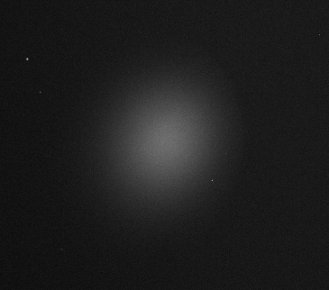
\includegraphics{fourier-020.jpg}};
  \draw [very thick, ->] (5.65,4.1) to [out=80, in=-10] (example.east);
\end{tikzpicture}

  \end{center}
\end{frame} 
